\chapter{Analisys and result discussion}
In the previous section the author has explained the steps followed to forecast electricity prices and explore the different predictors' influence. We are now discussing the configuration fixed for the hourly, daily, monthly and yearly setups, and the results obtained on each case.

The length of the time series to be used, the forecasting horizon, the number of lags and the predictors to be included have to be selected for each specific scenario. They have been chosen with the help of a topic expert, concretely my Thesis' Supervisor.

For the hourly and daily levels, the pre-pandemic and post-war markets are being studied.

\section{Hourly analysis}
In this case the author is working with a 6 months data window. It has been decided to make 168 hours ahead forecasts (1 week). The lags in use try to model the autocorrelation, and are the following: 1, 2, 12, 23, 24, 36, 71, 72, 167 and 168. Apart, other predictors are included to add extra information to the model:

\begin{itemize}
    \item \textbf{Date predictors:} Hour, day and day of week.
    \item \textbf{Demand:} The total energy demand.
    \item \textbf{Generation:} Wind, hydropower, nuclear, solar, combined cycle and coal generation technologies measurements.
\end{itemize}

Cross validation is applied using 15 windows, with step size of 191.

As the author mentioned, the energy market should have changed due to the Covid pandemic and specially to the war in Ukraine. These differences between current and past market will be analyzed.

\subsection{Pre-pandemic scenario}
The data used for the pre-pandemic scenario experiments goes from 2018-10-01 to 2019-03-31, before the increase in energy prices shown in Figure \ref{fig:spot-price-series-month}. In Table \ref{tab:cv-hourly-prep} you can find the performance of different models for the cross validation phase. The best one is a Random Forest, it is the one the author will use to make the final forecast.

\begin{table}[H]
\centering
\begin{tabular}{@{}l|l|l@{}}
\toprule
Model & MASE  & Modelling time (s)  \\ \midrule
RF    & 1.196 & 192.24              \\
GBT   & 1.264 & 113.17              \\
kNN   & 1.919 & 97.52               \\ \bottomrule
\end{tabular}
\caption{Model performance comparison trained over the hourly pre-pandemic energy price.}
\label{tab:cv-hourly-prep}
\end{table}

The final forecast is generated as explained in Chapter \ref{ch:methodology}, using the train split to build the model and the test to give a final estimation of the performance. The forecast is shown in Figure \ref{fig:forecast-hourly-pre}, obtaining a MASE of 1.18.

\begin{figure}[H]
\centering
    \caption{Final forecasting of hourly pre-pandemic energy price.}
    \label{fig:forecast-hourly-pre}
    \fbox{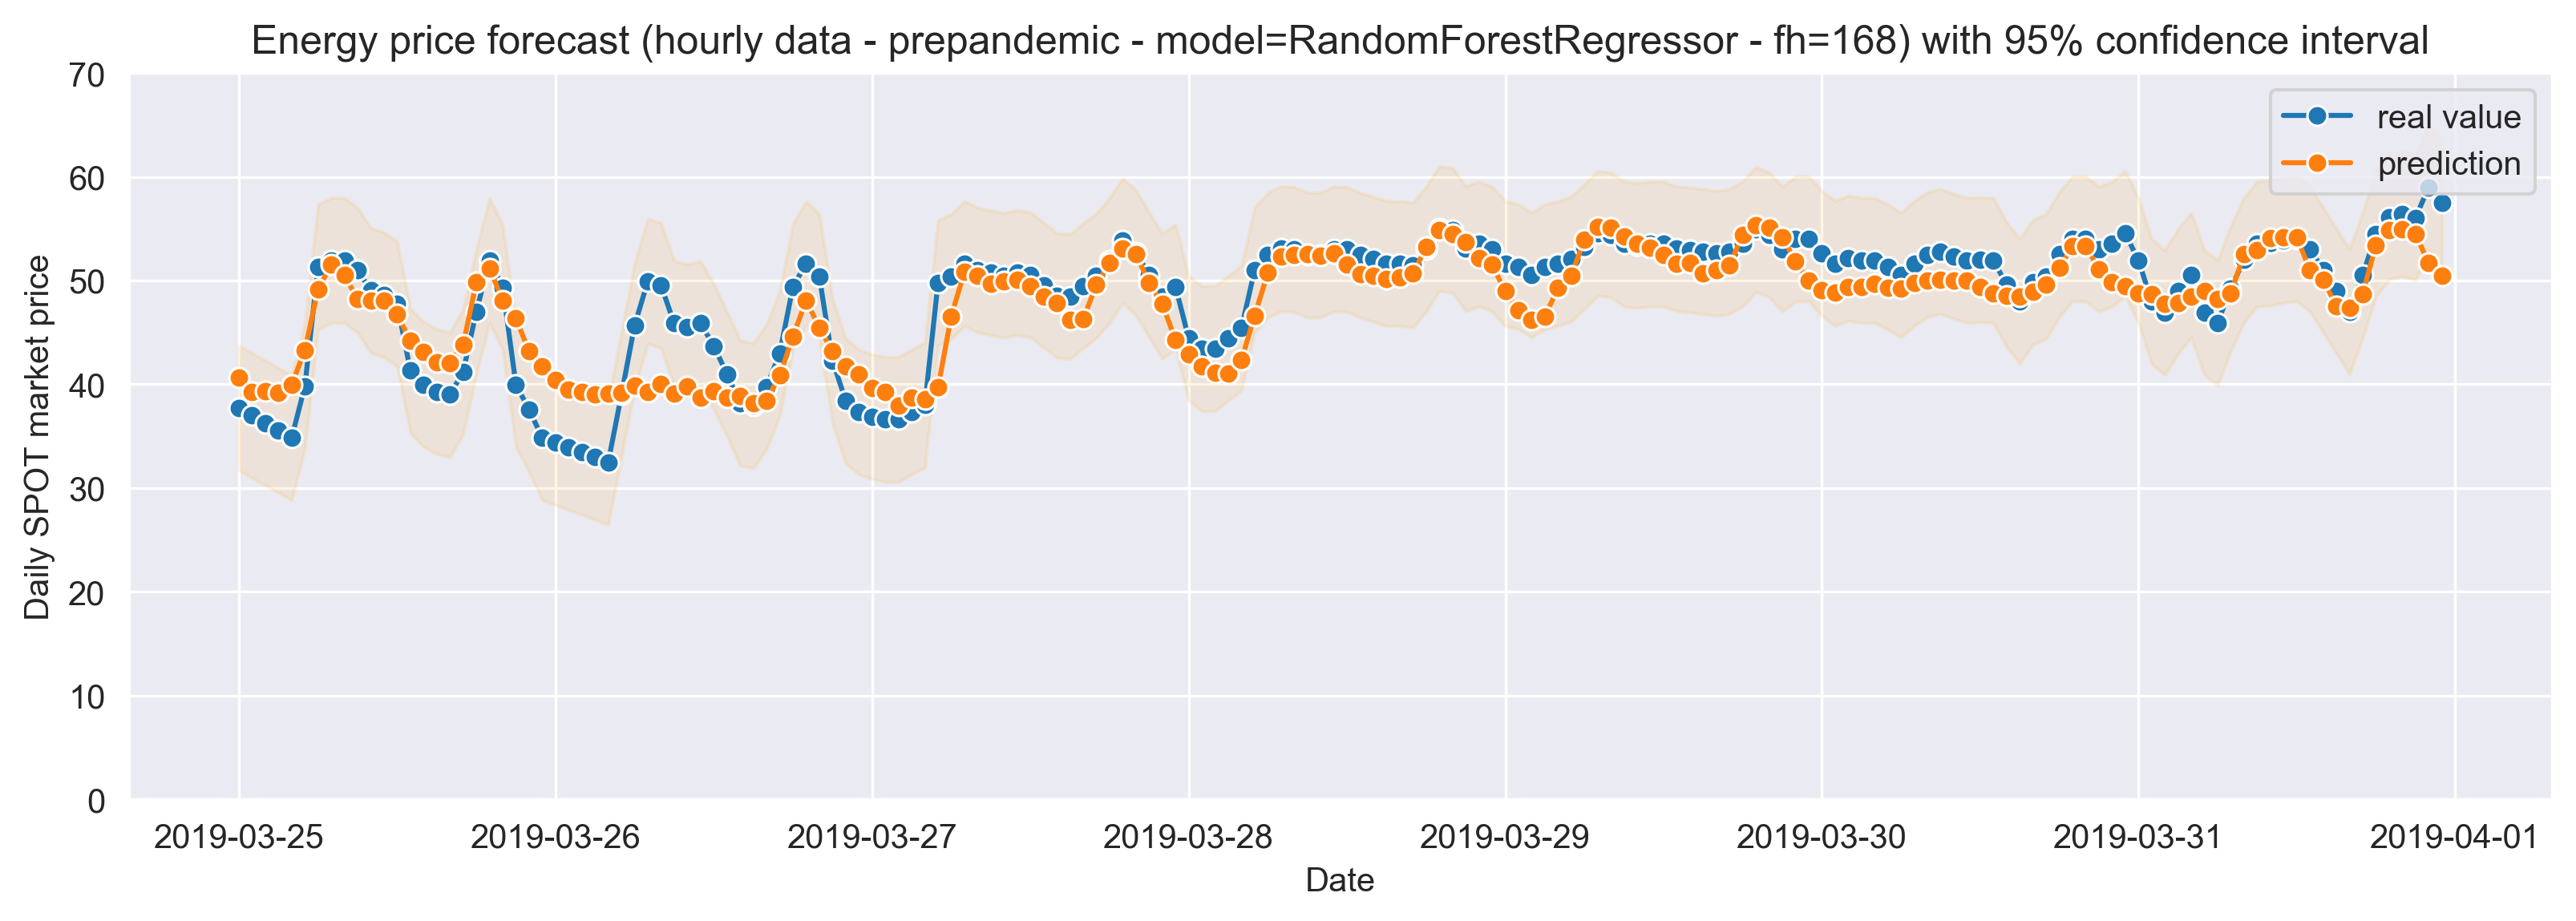
\includegraphics[scale=0.4]{images/analysis/forecast-hourly-pre}}
\end{figure}

Which are the predictors that are specially influencing this forecast? If lags are included in the SHAP study, see Figure \ref{fig:shap-hourly-pre-lags}, the first lag has a lot of importance. Concretely, if the lag takes a low value (blue color), the response value will tend to be low too, and vice-versa. Lag two has also some importance, but in this case a low value in the lag means a higher value in the response and vice-versa. The third lag with more importance is 167, specially in the positive side, when it takes a high value the output does the same.

About the rest of predictors, combined cycle generation and hour seem to have some importance. If the generation by combined cycle is high, the price goes up and vice-versa. The price in earlier hours is usually cheaper than in the end of the day: this makes sense, being correlated with the demand which is lower during the night.

Let's now train the same model without lags to see the predictor's importance more clearly (Figure \ref{fig:shap-hourly-pre-nolags}). Again, combined cycle generation and hour are between the most influential predictors. Others such as coal, nuclear and hydropower generation appear in the top too. For the nuclear case, the more generation the lower the energy price: as explained in Chapter \ref{ch:electricity-market}, nuclear plants can't be stopped, so they always bet for very low prices. The more nuclear generation, the higher the chances of getting a low price.

\begin{figure}[H]
\centering
    \begin{subfigure}[t]{.45\textwidth}
        \centering
        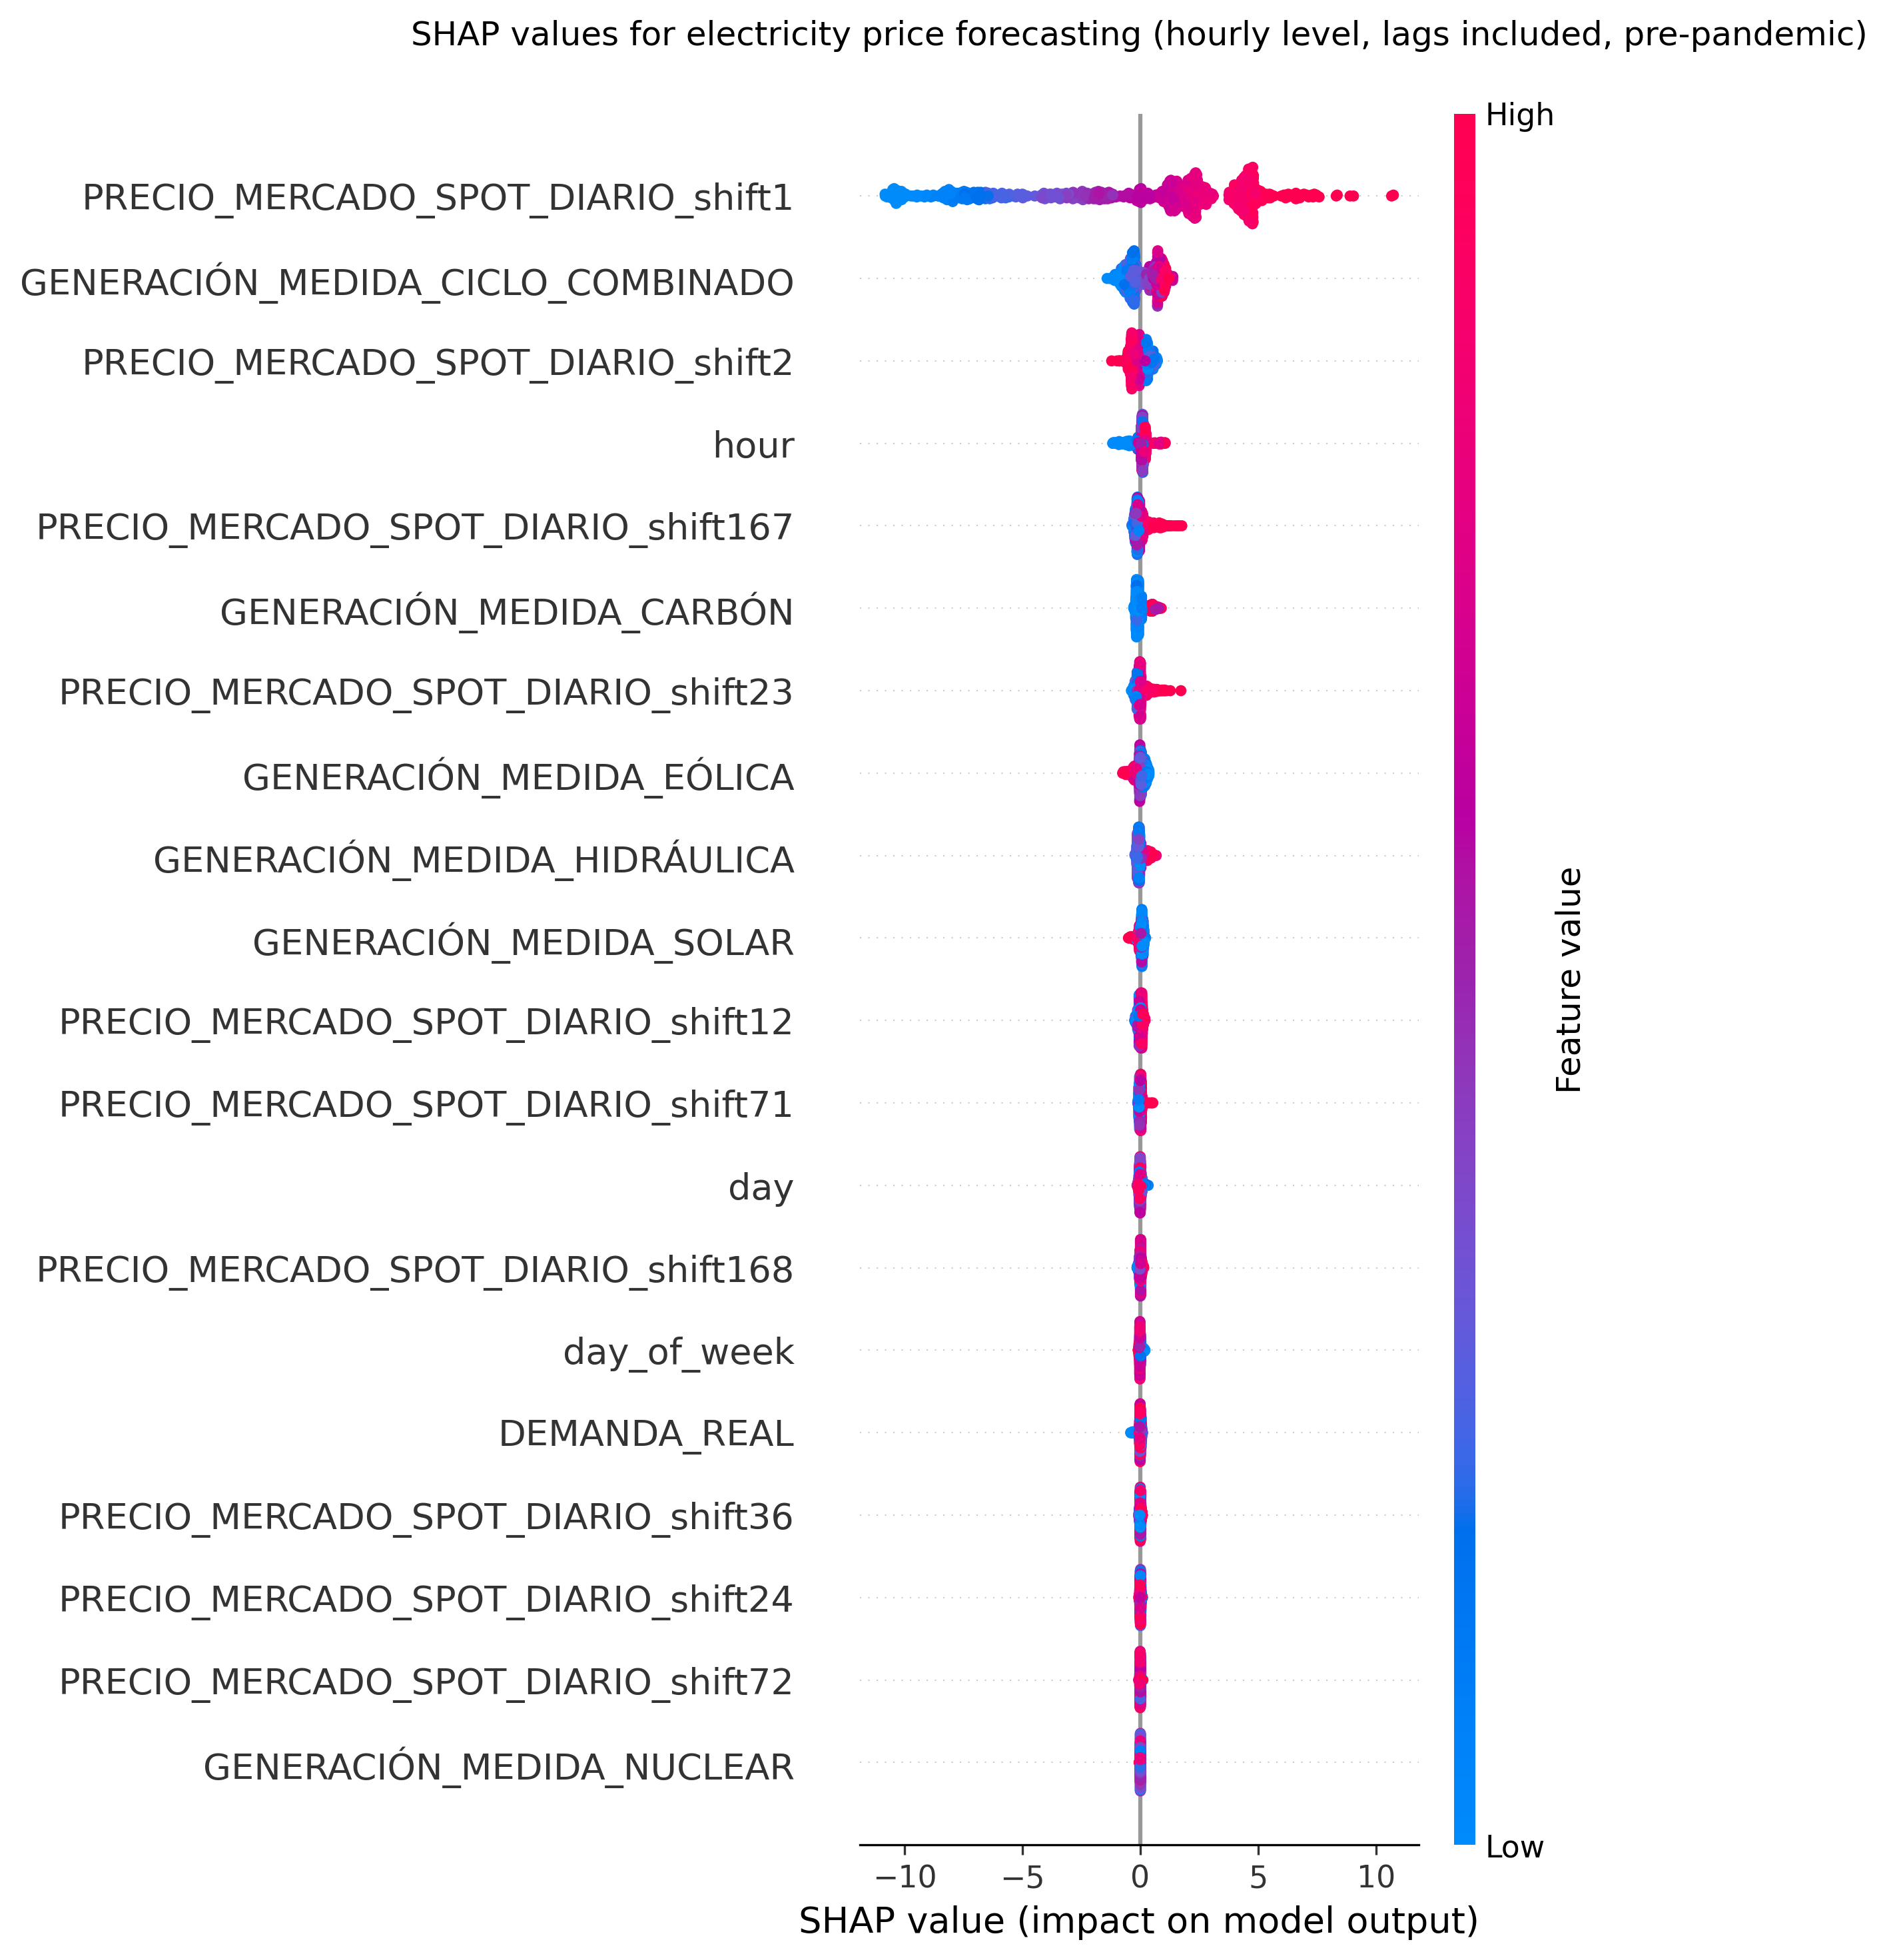
\includegraphics[width=1\linewidth]{images/analysis/shap-hourly-pre}
        \caption{SHAP values including lags.}
        \label{fig:shap-hourly-pre-lags}
    \end{subfigure}
    \begin{subfigure}[t]{.45\textwidth}
        \centering
        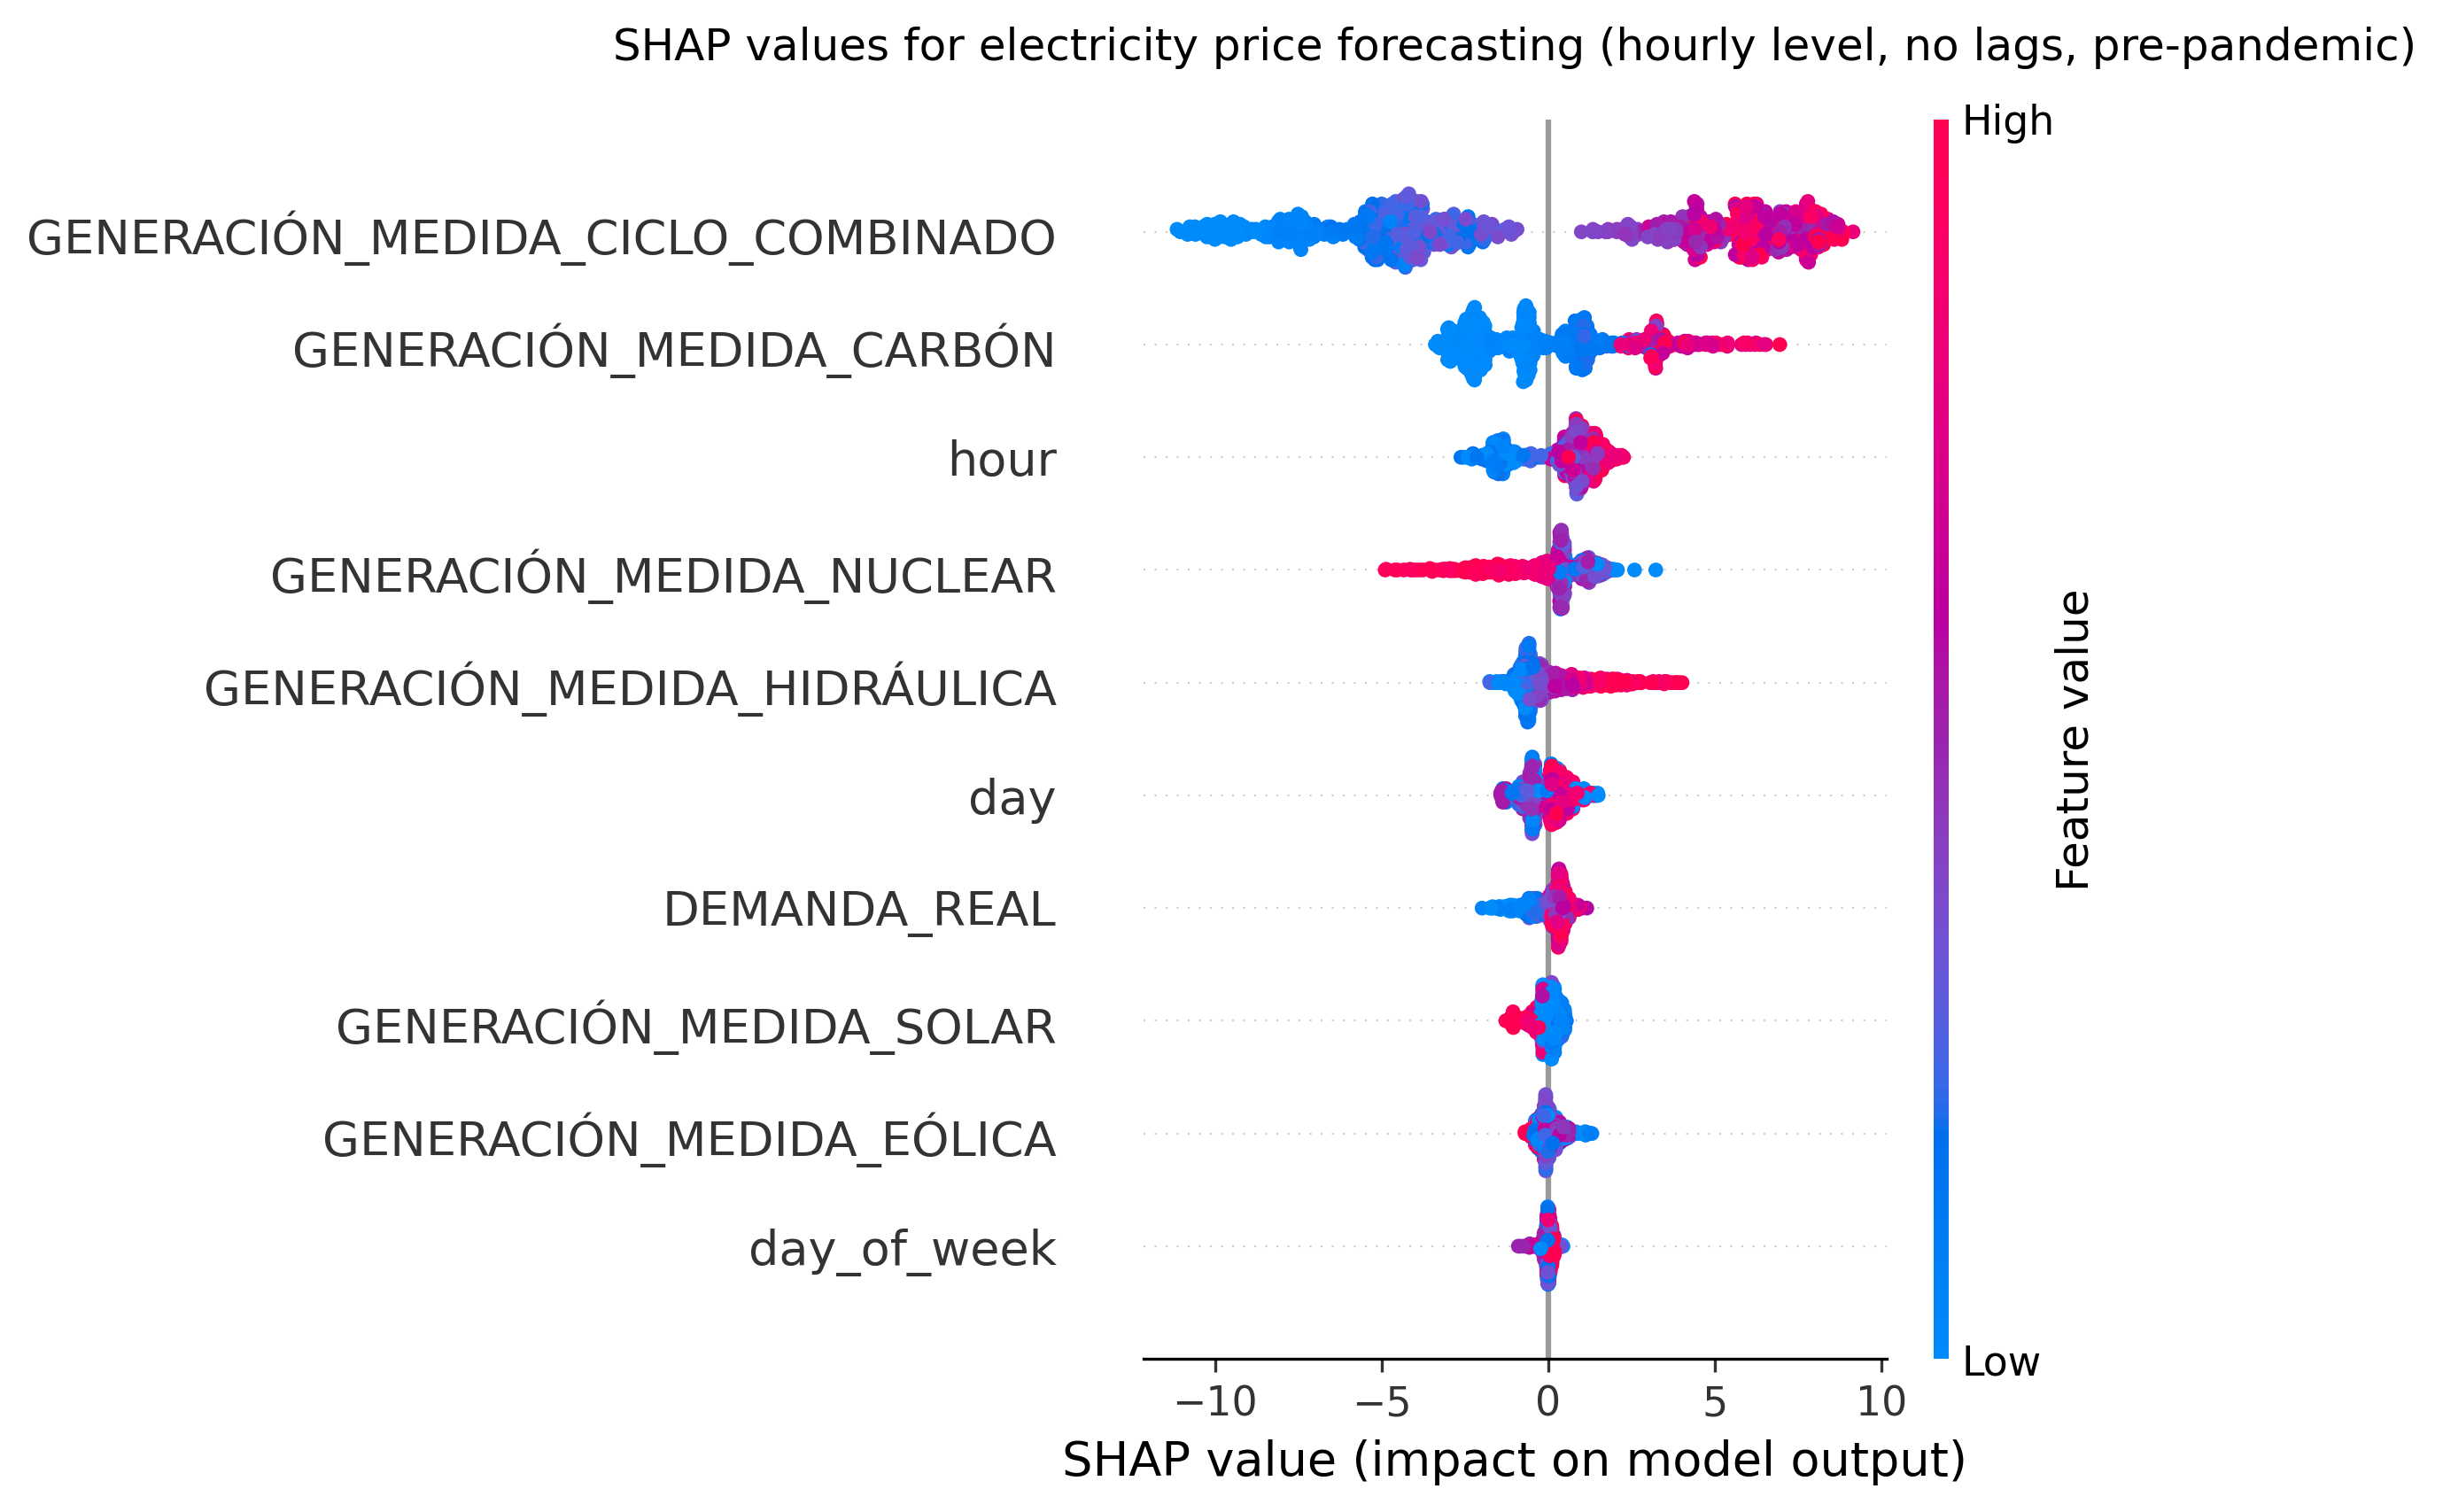
\includegraphics[width=1\linewidth]{images/analysis/shap-hourly-pre-nolags}
        \caption{SHAP values not including lags.}
        \label{fig:shap-hourly-pre-nolags}
    \end{subfigure}

    \caption{SHAP values for the hourly pre-pandemic energy price forecasting.}
    \label{fig:shap-hourly-pre}
\end{figure}

\subsection{Post-Ukraine war scenario}
The data in use goes from 2022-10-01 to 2023-03-31. In the model selection stage the author obtains the results described in Table \ref{tab:cv-hourly-post}.

% Please add the following required packages to your document preamble:
% \usepackage{booktabs}
\begin{table}[H]
\centering
\begin{tabular}{@{}l|l|l@{}}
\toprule
Model & MASE  & Modelling time (s)  \\ \midrule
RF    & 1,964 & 98.63               \\
GBT   & 2.081 & 67.17               \\
kNN   & 4.014 & 111.84              \\ \bottomrule
\end{tabular}
\caption{Model performance comparison trained over the hourly post-Ukraine war energy prices.}
\label{tab:cv-hourly-post}
\end{table}

The best-performing model, in this post-war scenario, is again the one based on Random Forests (RF). The final forecast is shown in Figure \ref{fig:forecast-hourly-post}: a final MAE of 1.702 has been obtained over the test partition. It can be checked how the model is correctly capturing the cyclicity in the data.

\begin{figure}[H]
\centering
    \caption{Final forecasting of hourly post-war energy price.}
    \label{fig:forecast-hourly-post}
    \fbox{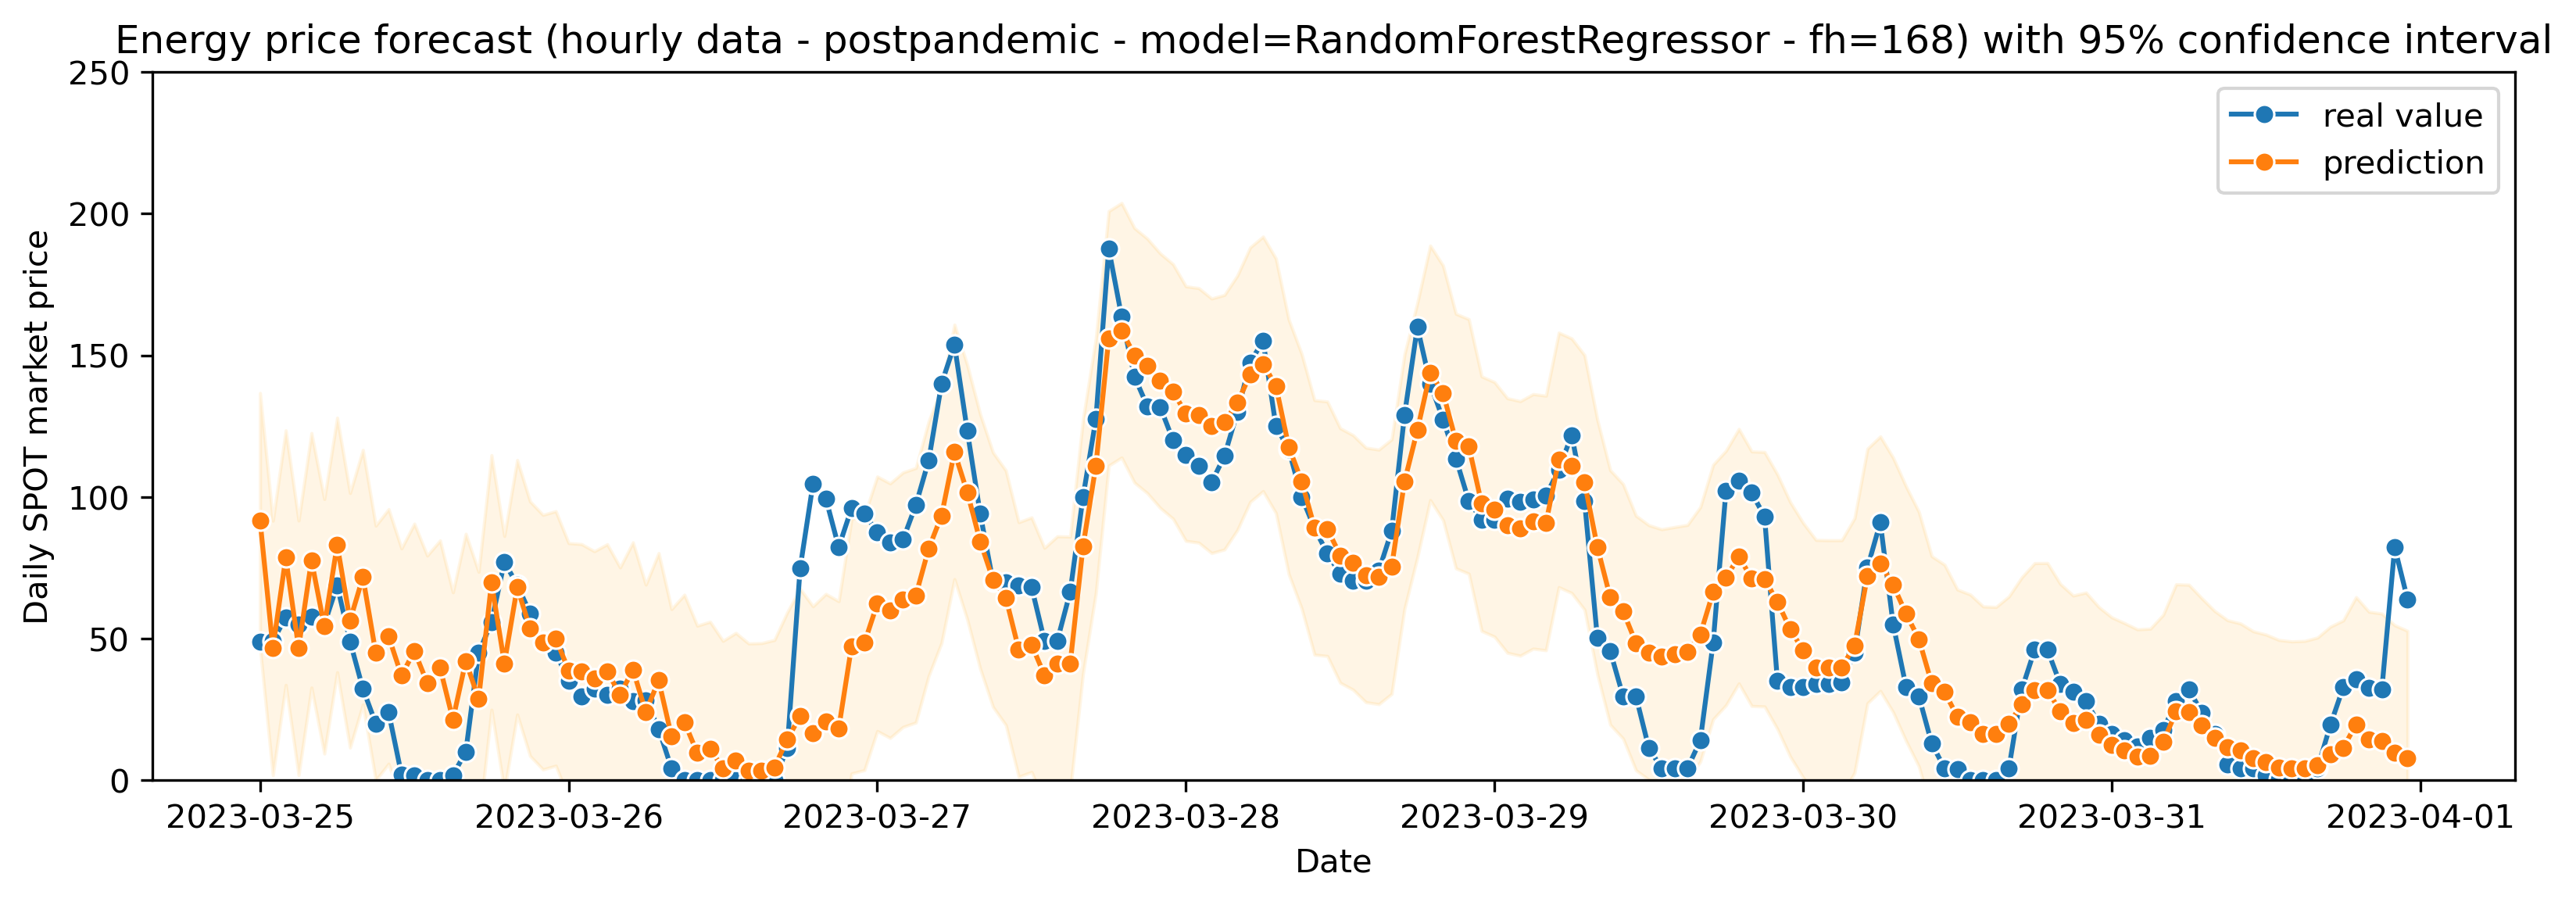
\includegraphics[scale=0.4]{images/analysis/forecast-hourly-post}}
\end{figure}

In this case, the most important predictors are shown in Figure \ref{fig:shap-hourly-post}. Compared with the pre-pandemic series, we find similar predictors. A lag which seems more important than before is 23, but in general everything is similar.

If the model without using lags is studied, the most influential variable is again combined cycle generation. It seems to be more influential than before, relatively comparing with other predictors' importance. Date predictors such as day, day or week or hour are also relevant and others such as demand, hydropower and nuclear generation.

An interesting point here is how coal generation has lost importance compared to previous years: this makes sense, as coal is less and less used as it is highly polluting. Check Figure \ref{fig:coal-series} and see how is almost irrelevant from 2019 onwards.

\begin{figure}[H]
\centering
    \begin{subfigure}{.45\textwidth}
        \centering
        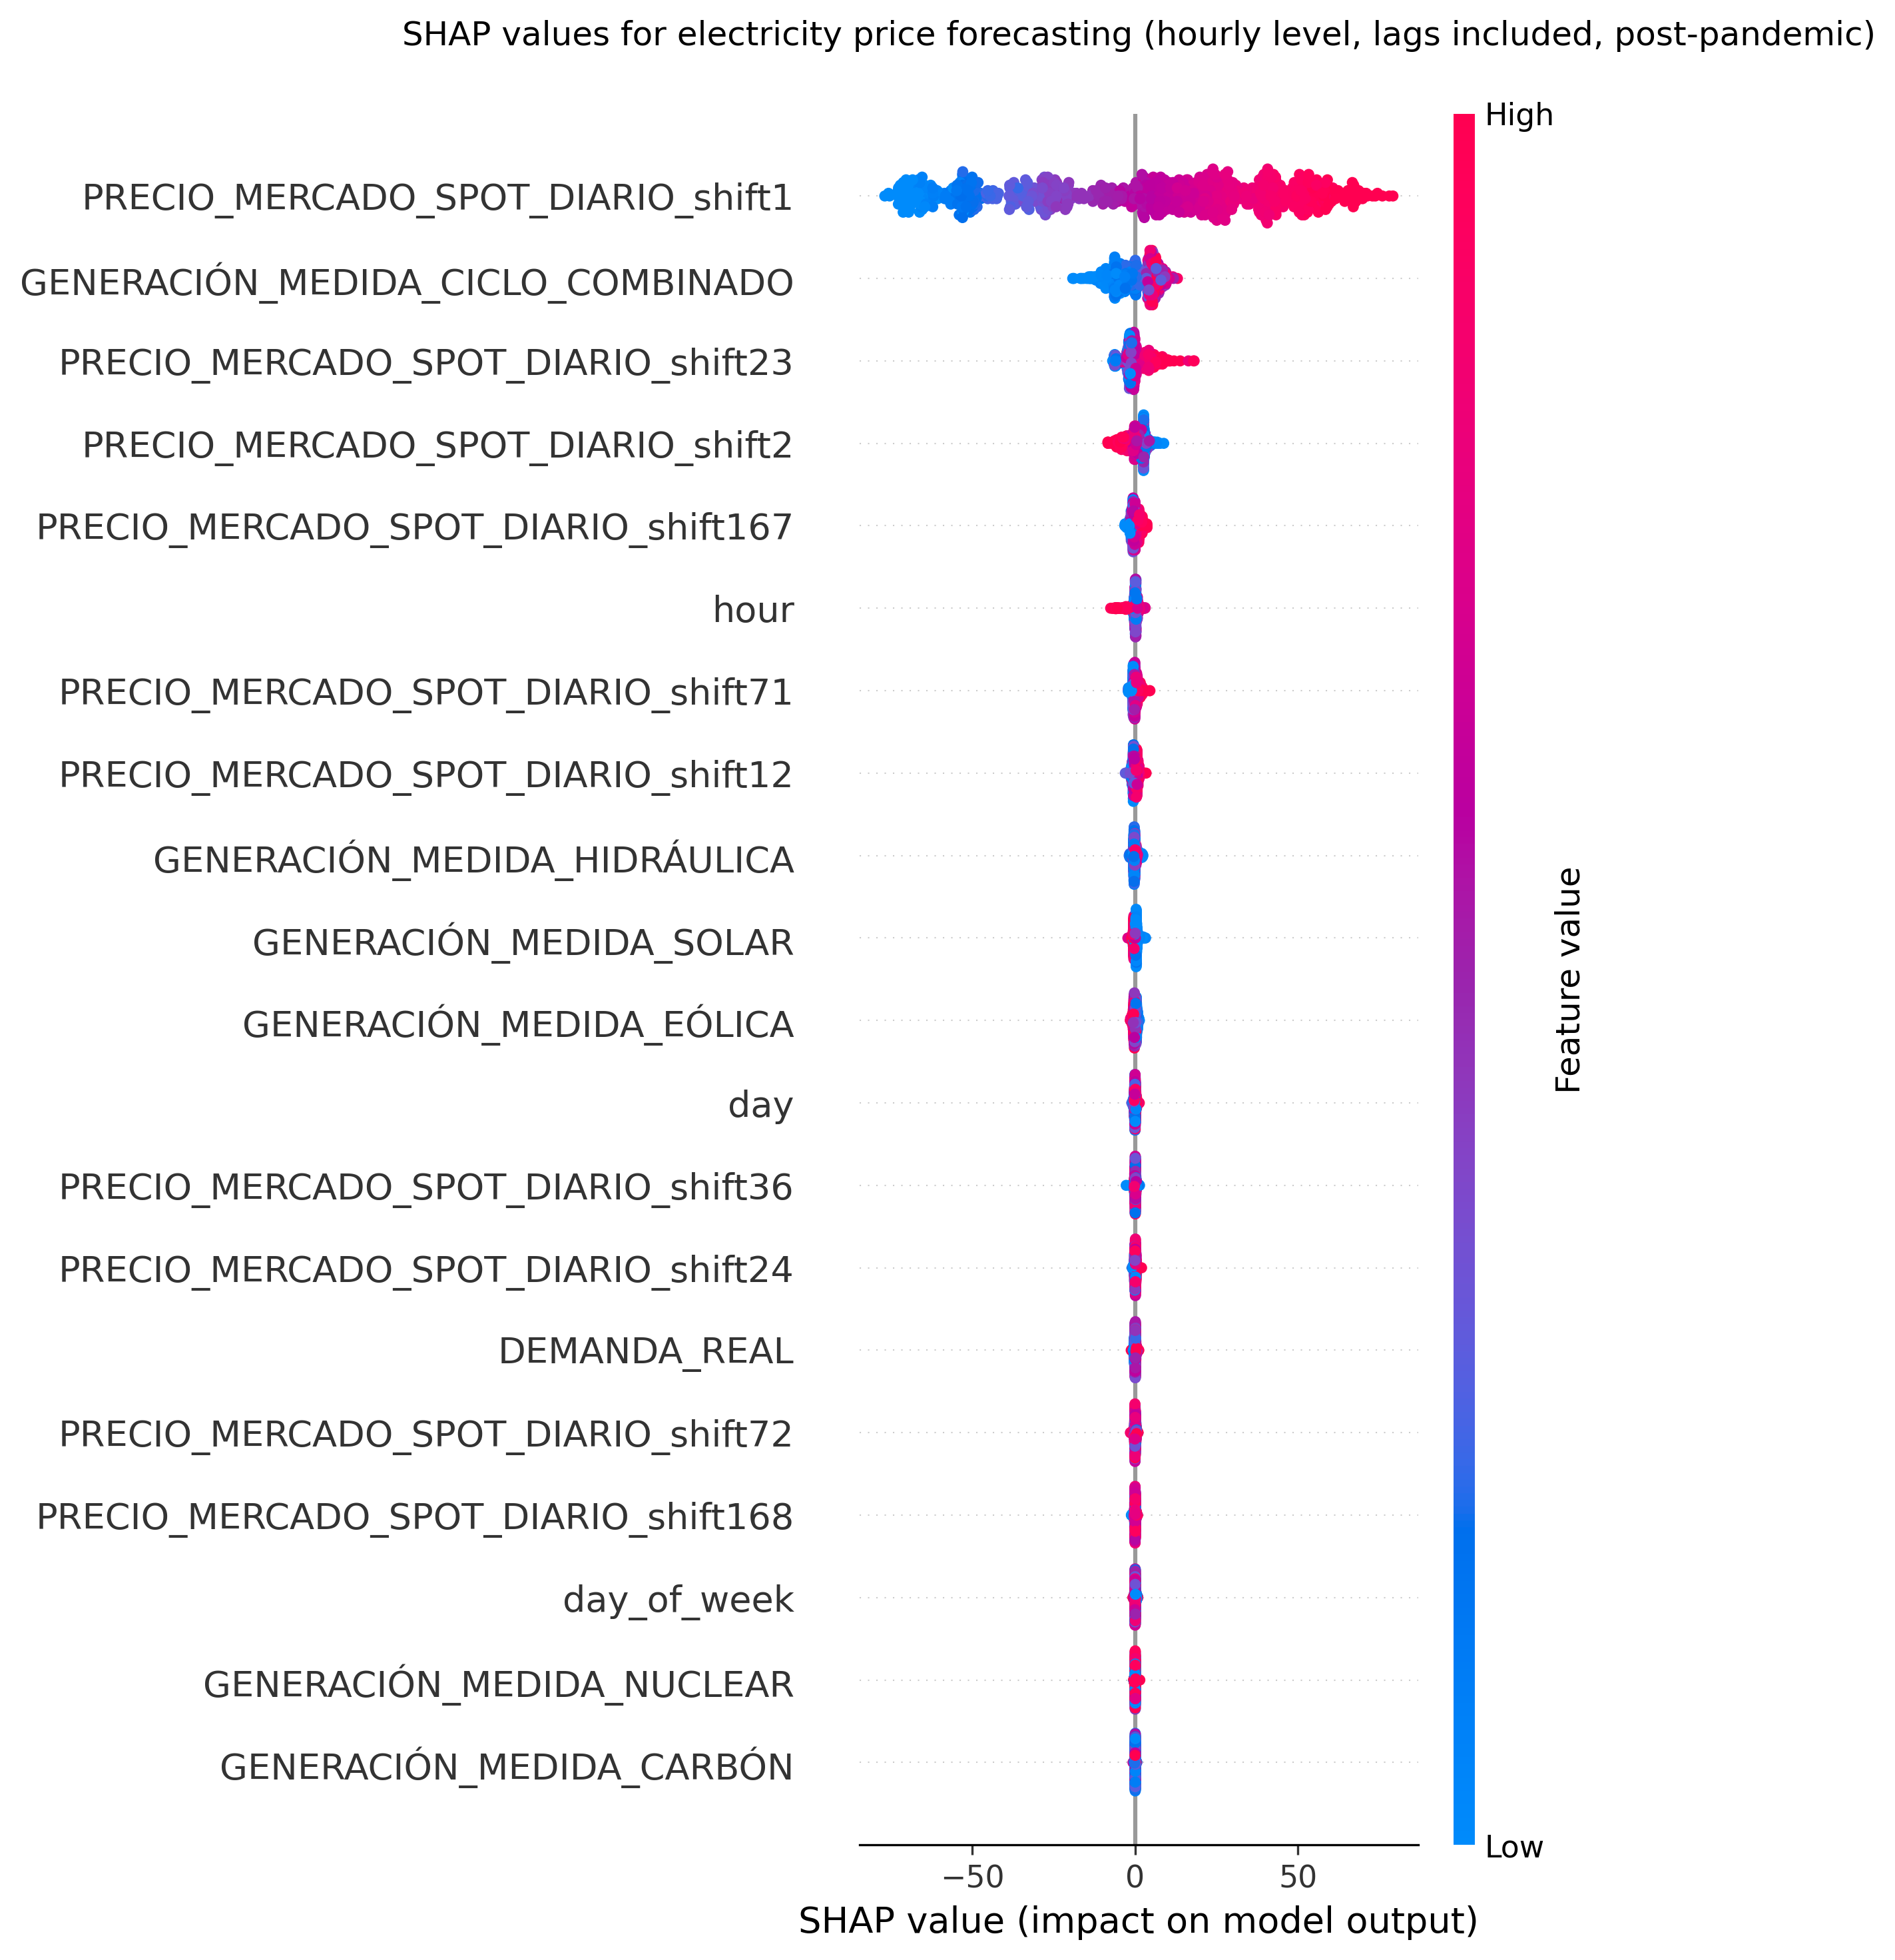
\includegraphics[width=1\linewidth]{images/analysis/shap-hourly-post}
        \caption{SHAP values including lags as predictors.}
        \label{fig:shap-hourly-post-lags}
    \end{subfigure}
    \begin{subfigure}{.45\textwidth}
        \centering
        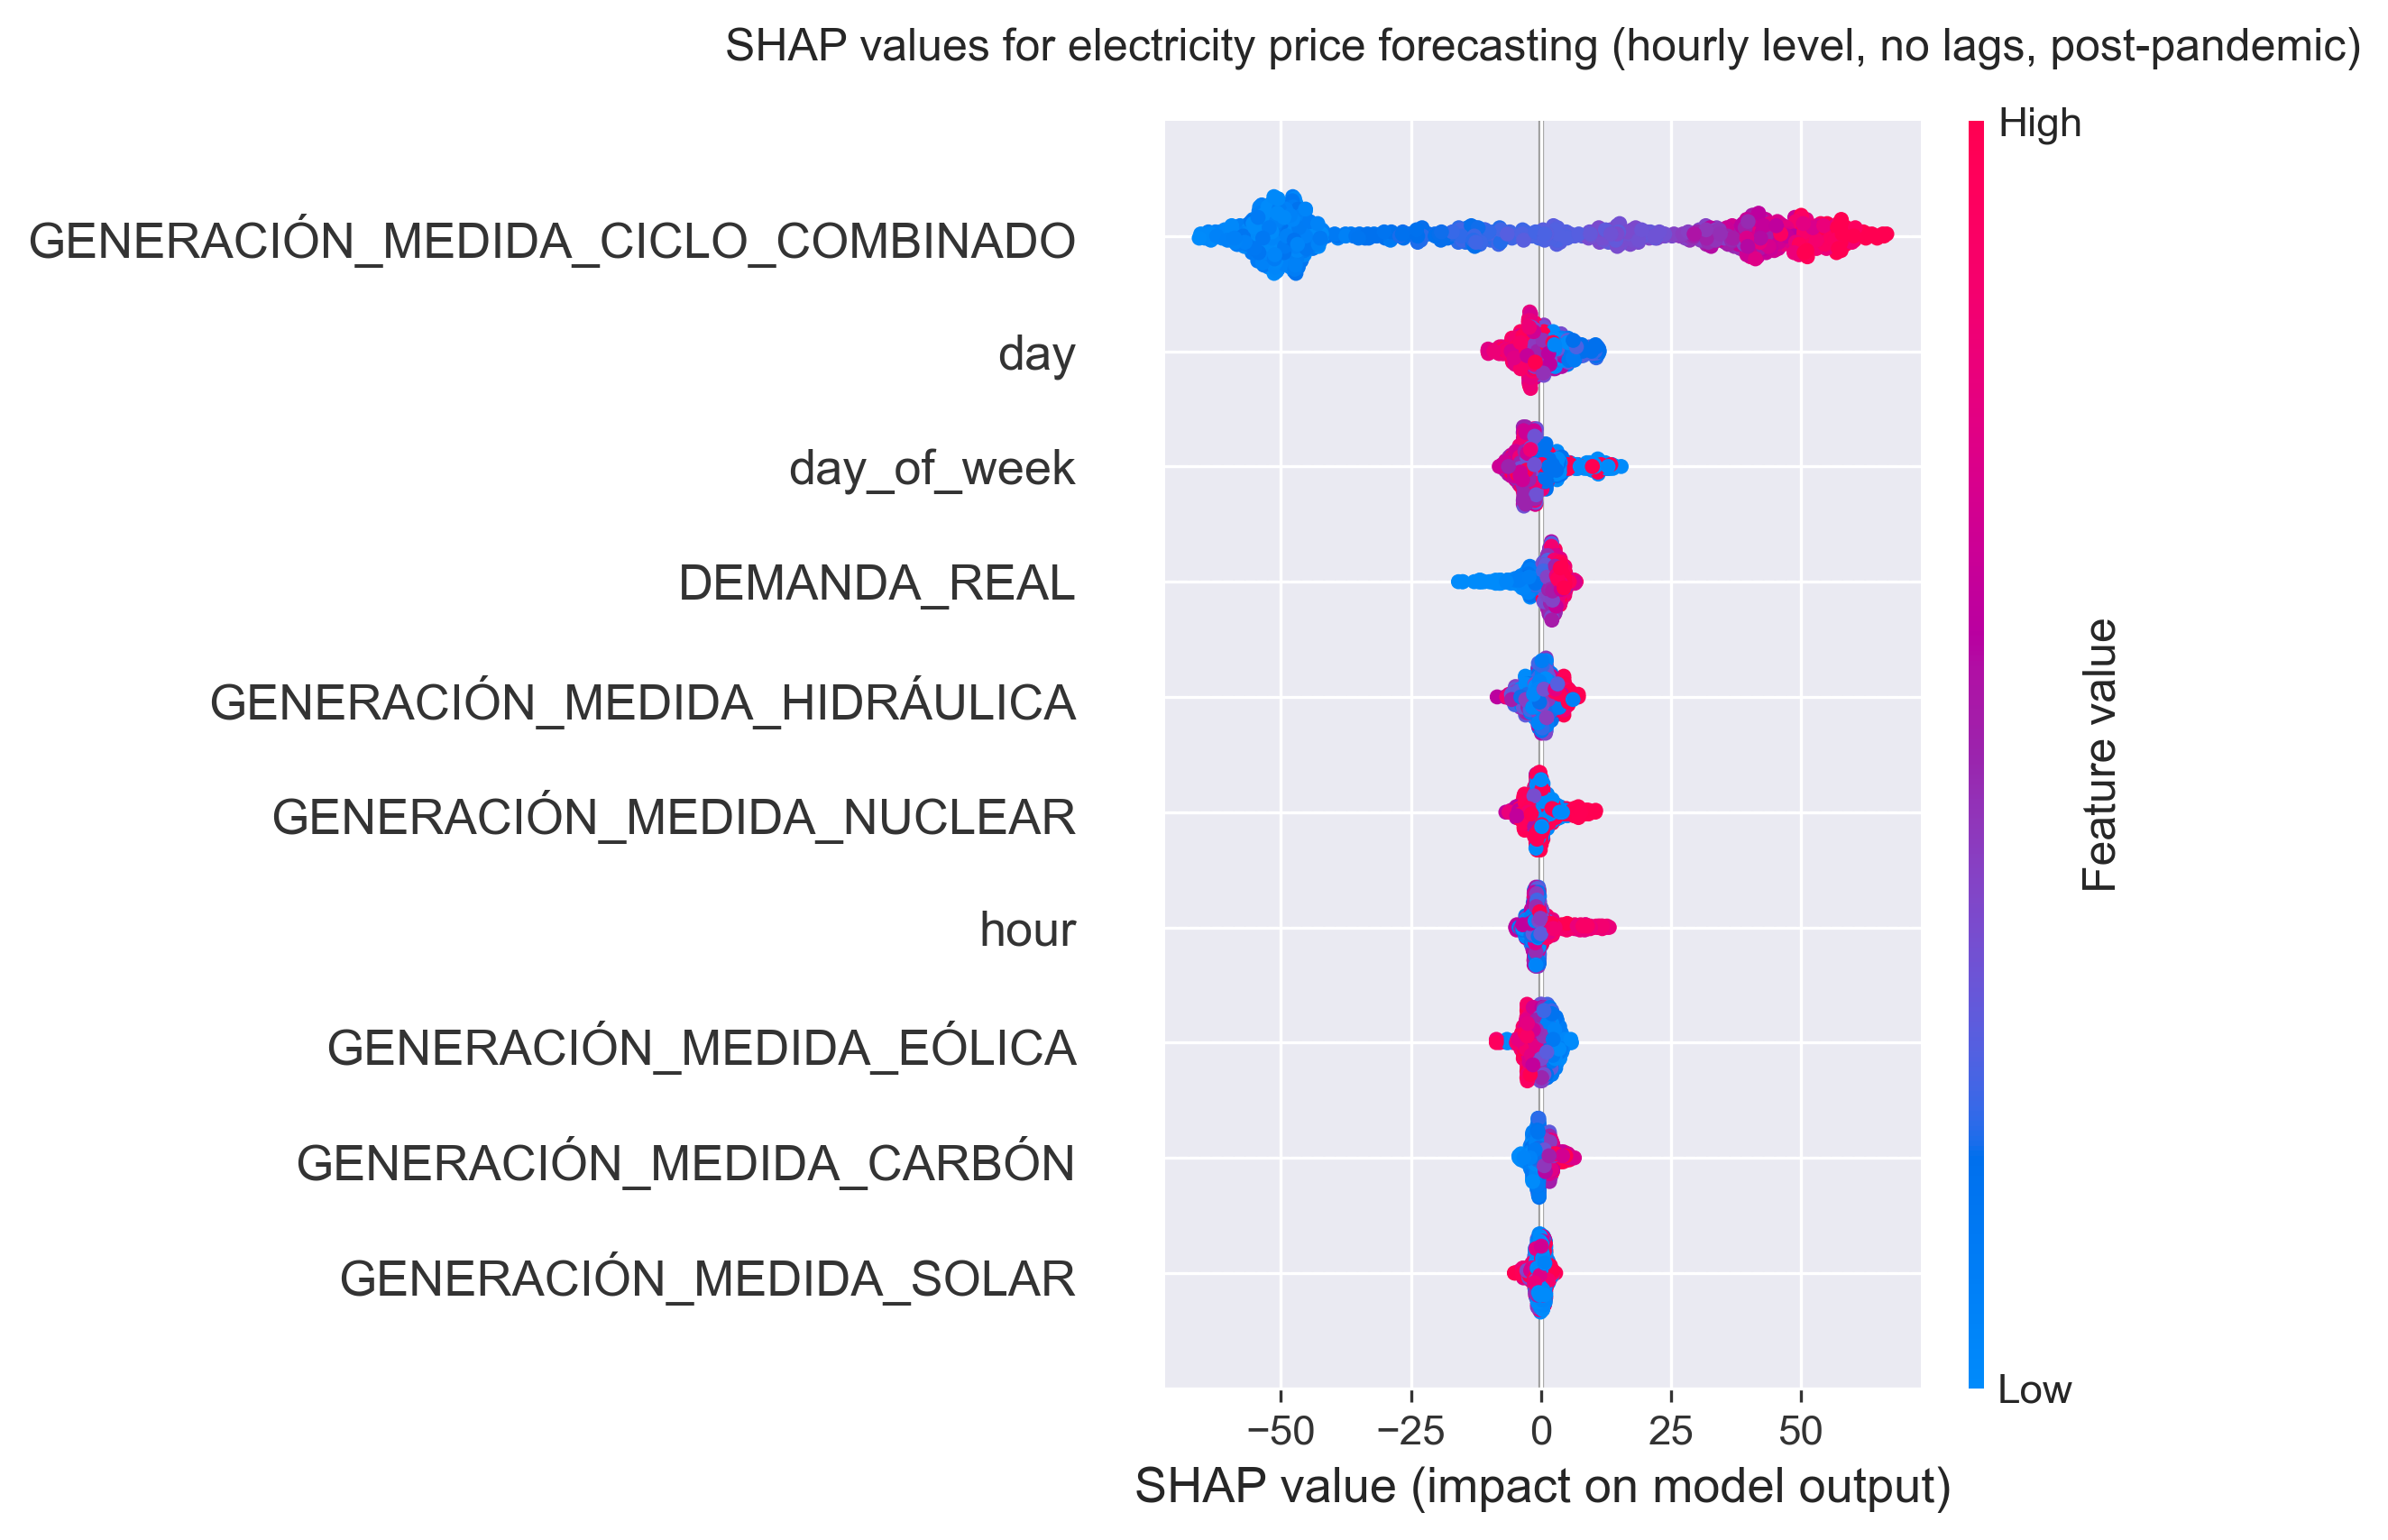
\includegraphics[width=1\linewidth]{images/analysis/shap-hourly-post-nolags}
        \caption{SHAP values not including lags as predictors.}
        \label{fig:shap-hourly-post-nolags}
    \end{subfigure}

    \caption{SHAP values for the hourly post-pandemic energy price forecasting.}
    \label{fig:shap-hourly-post}
\end{figure}

\subsection{Result discussion}
Both for the pre-pandemic and post-war scenarios the best performing models are Random Forests. Looking at the forecasts graphs, they are correctly capturing the cyclicity present in data.

An important conclusion on this study is that combined cycle generation is a relevant predictor to model hourly prices. This makes sense, because as described in Chapter \ref{ch:electricity-market}, the commodity-based technologies normally set the energy price. In the post-war market it has even gained more importance. Also, it can be seen how coal generation has lost importance in the past years, to the extent that it is hardly used today.


\newpage
\section{Daily analysis}
For the daily aggregation analysis 2 years of data are used, producing 30 days ahead forecasts. The lags added as predictors are 1, 2, 6, 7, 13, 14, 28, 30 and 31, apart we use the following new predictors:

\begin{itemize}
    \item \textbf{Date predictors:} Day, day of week, week of the year and month.
    \item \textbf{Gas price}
    \item \textbf{Coal price}
    \item \textbf{EU $CO_2$ allowances price}
\end{itemize}

\noindent Cross validation is applied again using 15 windows, but in this case the step size is 13.

\subsection{Pre-pandemic scenario}
The data used for the pre-pandemic scenario experiments ranges from 2018-04-01 to 2020-03-31. The model which performed the best was based on Gradient Boosting Trees (GBT), obtaining 1.044 as MASE, as can be seen in Table \ref{tab:cv-daily-prep}.

\begin{table}[H]
\centering
\begin{tabular}{@{}l|l|l@{}}
\toprule
Model & MASE  & Modelling time (s)  \\ \midrule
GBT   & 1.394 & 110.12 \\
RF    & 1.579 & 99.21  \\
kNN   & 1.965 & 156.20 \\ \bottomrule
\end{tabular}
\caption{Model performance comparison trained over the daily pre-pandemic energy price.}
\label{tab:cv-daily-prep}
\end{table}

The final forecast generated using GBT over holdout returns a MASE score of 1.043. The result can be visualized in Figure \ref{fig:forecast-daily-pre}: most of the true values remain inside the confidence interval generated during the forecast.

\begin{figure}[H]
\centering
    \caption{Final forecasting of daily pre-pandemic energy price.}
    \label{fig:forecast-daily-pre}
    \fbox{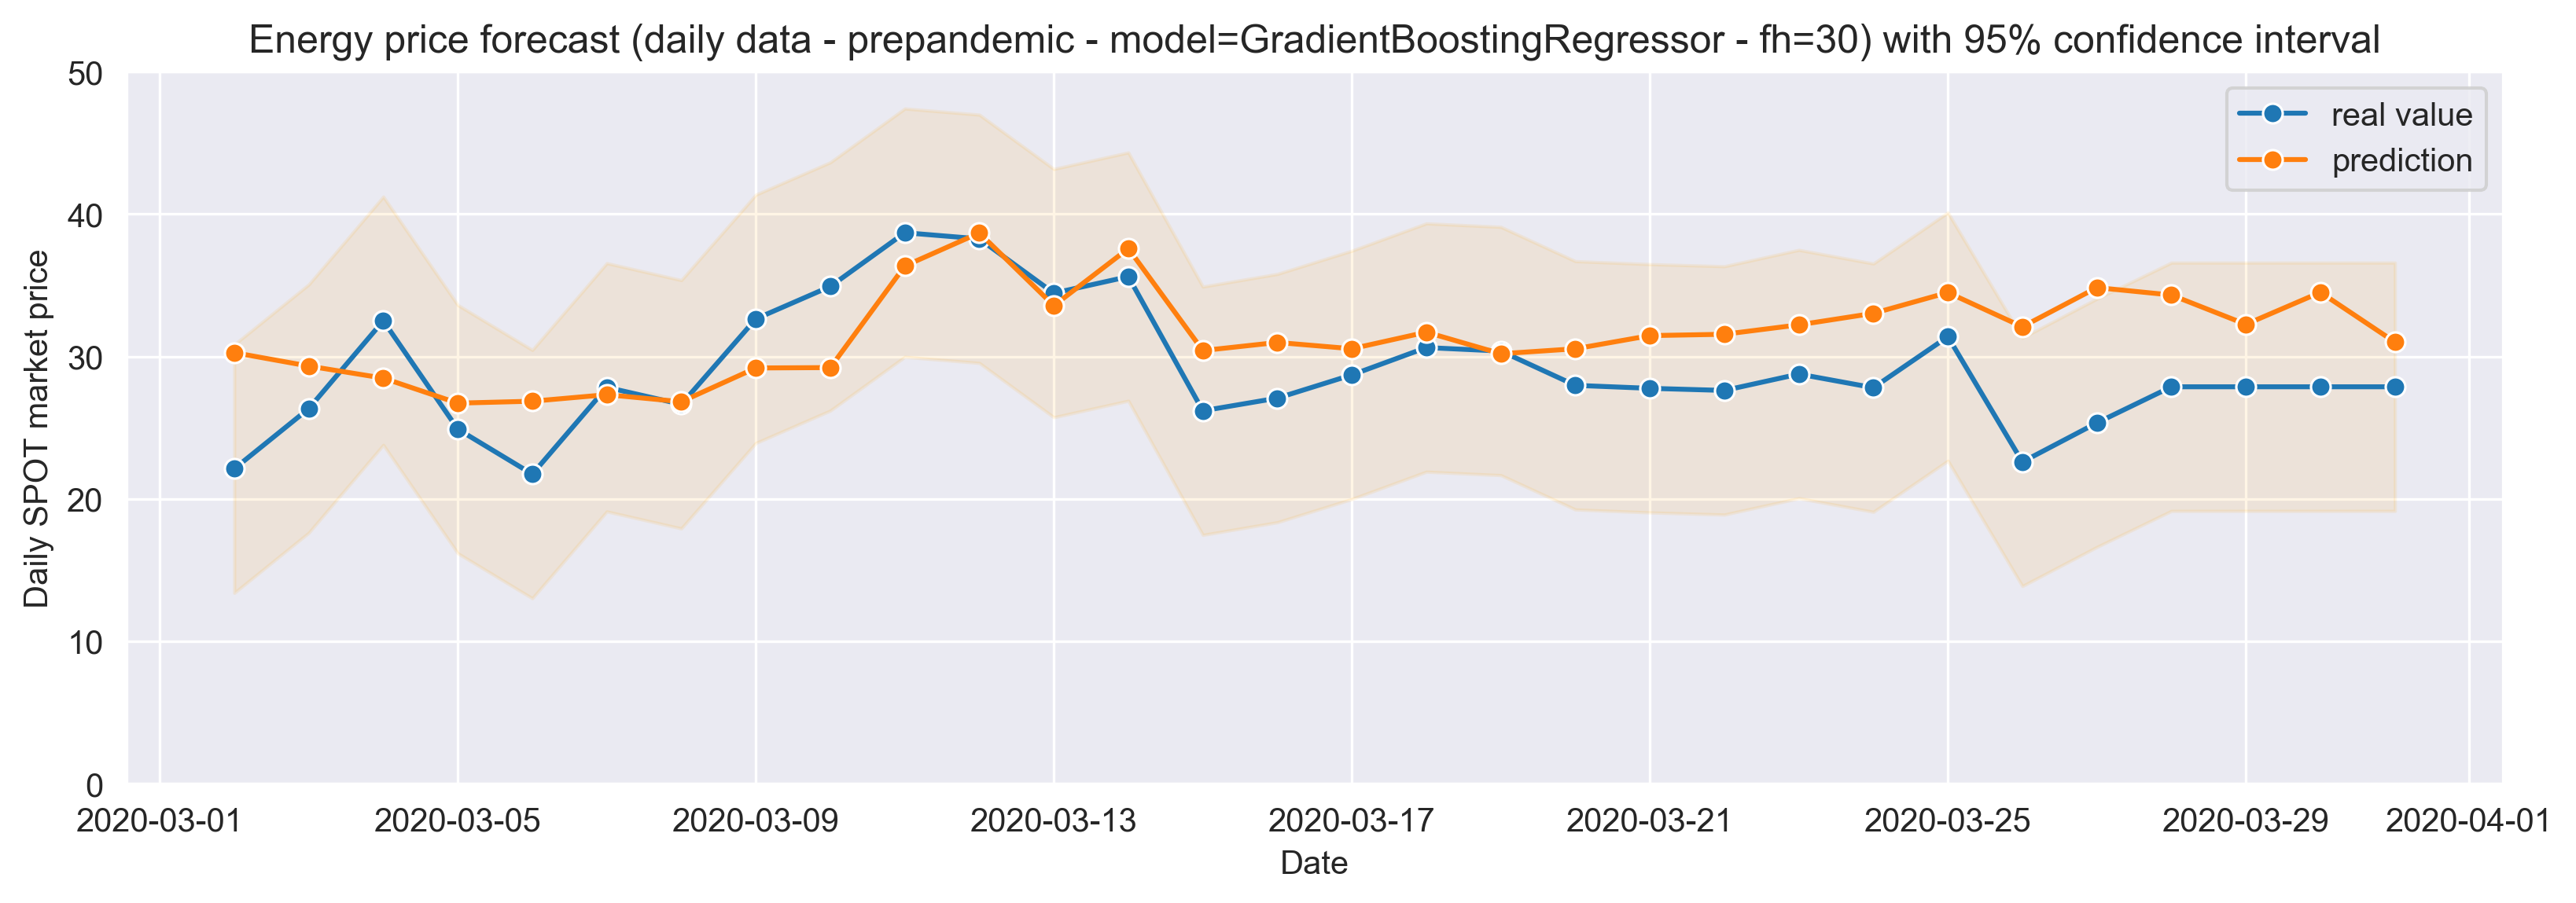
\includegraphics[scale=0.4]{images/analysis/forecast-daily-pre}}
\end{figure}

Let's now compute the SHAP values for this model. Again, we will analyze the case in which we use all the predictors (including lags) and the situation in which lags are excluded.

\begin{figure}[H]
\centering
    \begin{subfigure}{.45\textwidth}
        \centering
        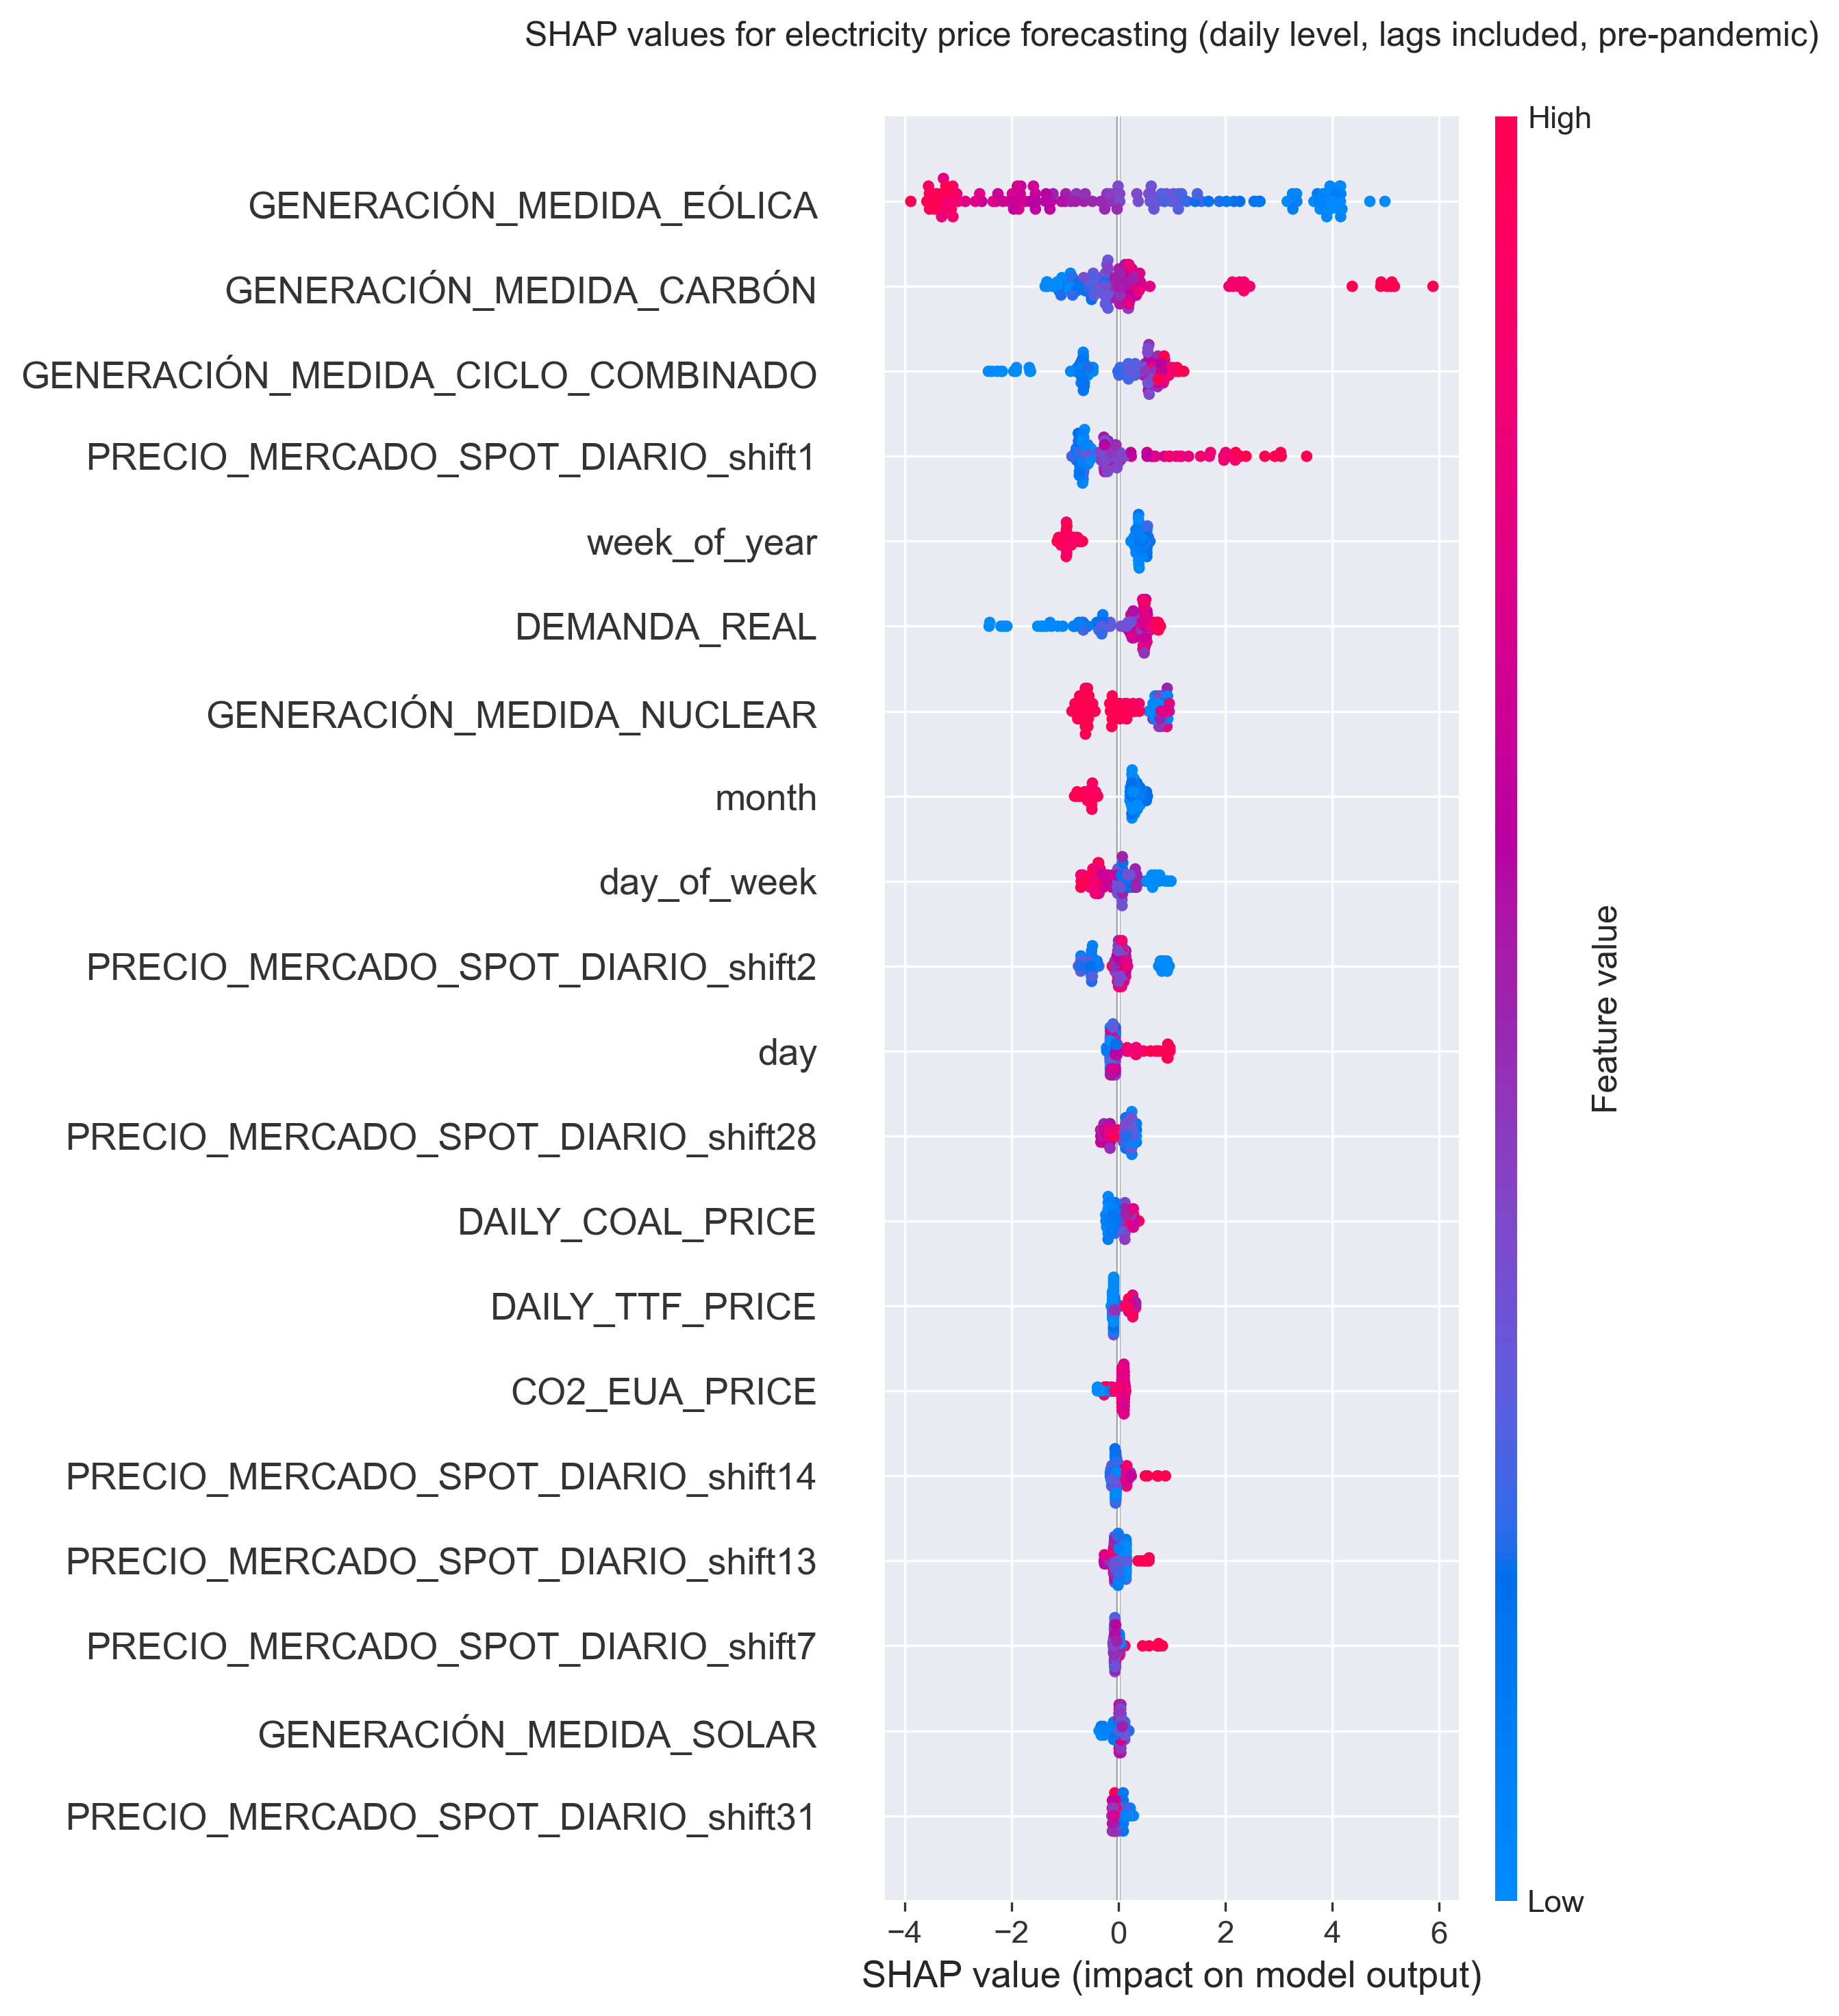
\includegraphics[width=1\linewidth]{images/analysis/shap-daily-pre}
        \caption{fh=1}
    \end{subfigure}
    \begin{subfigure}{.45\textwidth}
        \centering
        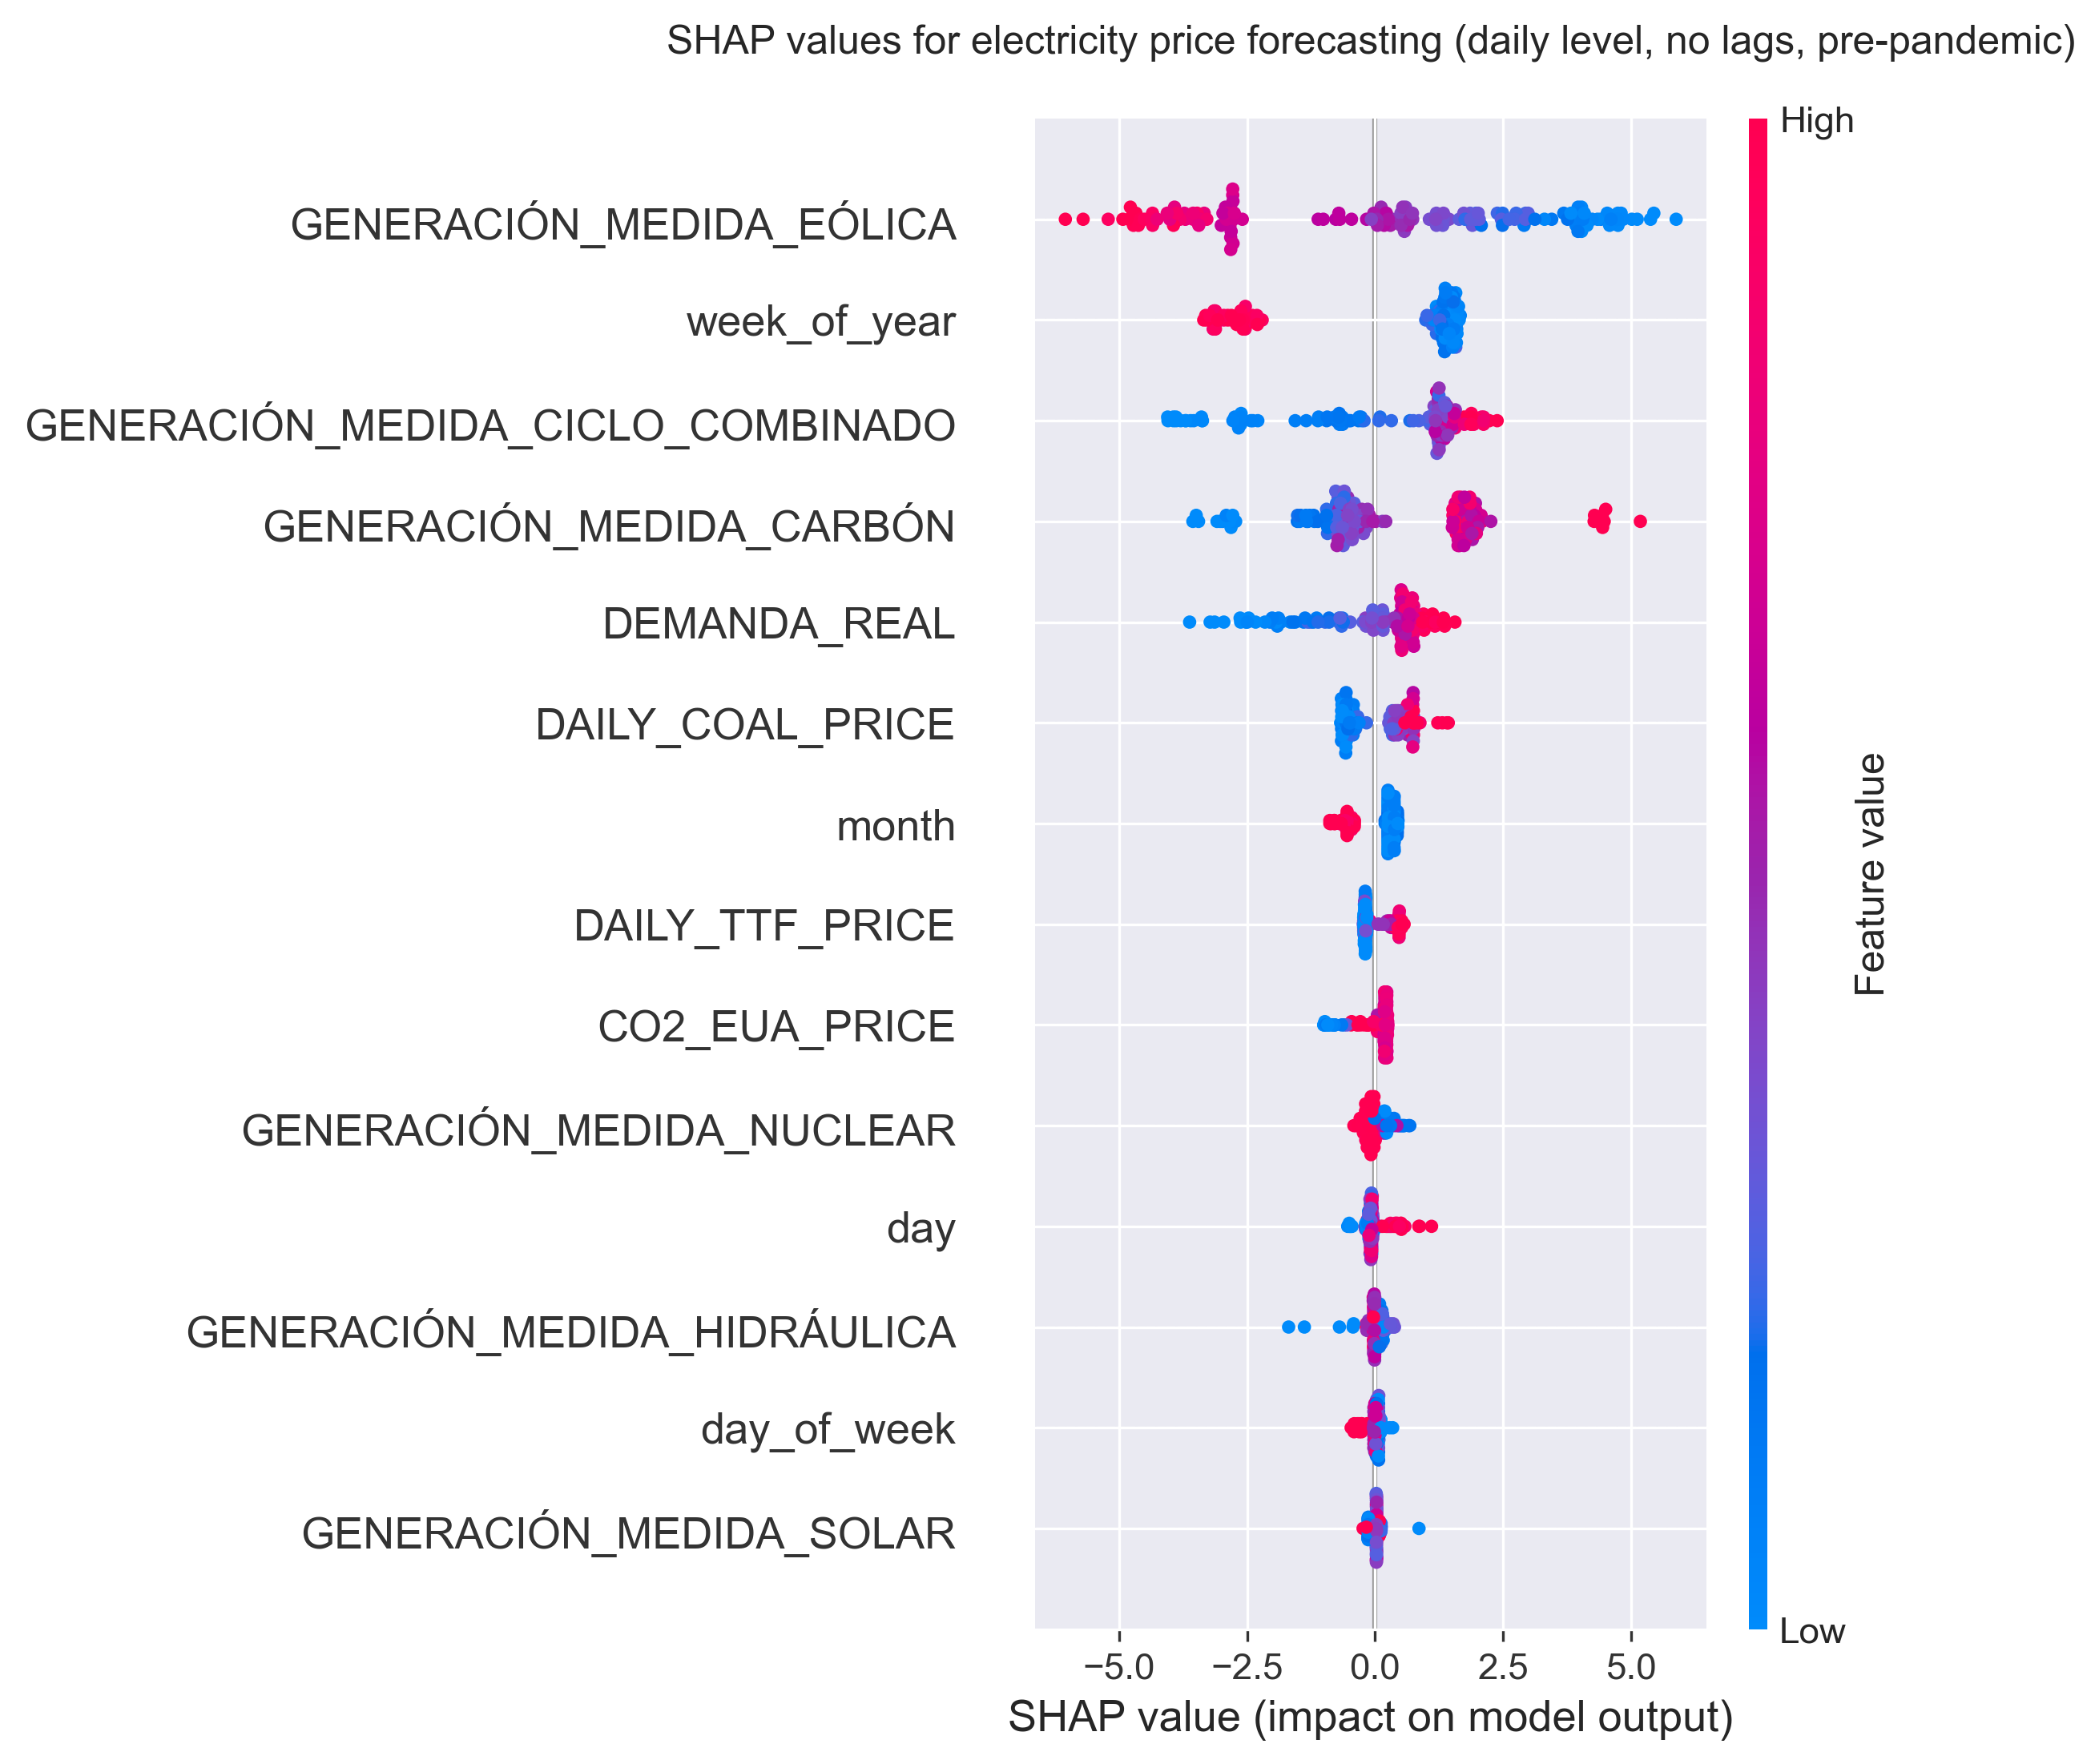
\includegraphics[width=1\linewidth]{images/analysis/shap-daily-pre-nolags}
        \caption{fh=30}
    \end{subfigure}

    \caption{SHAP values for the daily pre-pandemic energy price forecasting.}
    \label{fig:shap-daily-pre}
\end{figure}

We see how wind power, coal and combined cycle generation are the predictors influencing the forecast the most. As can be checked, high levels of wind power generation tend to lower the electricity price, while high level of combined cycle or coal generation tend to increase it. Between the date predictors, the one which stands out the most is the week of the year. Finally, the most important lag is 1, something that makes sense as is the closest to the response.

\subsection{After-Unkraine war scenario}
Let's now explore the after-war scenario. Data in use ranges from 2021-04-01 to 2023-03-31, and the best performing model changes to RF as seen in Table \ref{tab:cv-daily-post}.

\begin{table}[H]
\centering
\begin{tabular}{@{}l|l|l@{}}
\toprule
Model & MASE  & Modelling time (s)  \\ \midrule
RF    & 1.936 & 104.51  \\
GBT   & 2.153 & 67.30   \\
kNN   & 2.334 & 140.16  \\ \bottomrule
\end{tabular}
\caption{Model performance comparison trained over the daily post-war energy price.}
\label{tab:cv-daily-post}
\end{table}

After training RF with the complete cross-validation data and assessing the performance over the test partition, the MASE obtained is of 1.585. The result is shown in Figure \ref{fig:forecast-daily-post}.

\begin{figure}[H]
\centering
    \caption{Final forecasting of daily post-war energy price.}
    \label{fig:forecast-daily-post}
    \fbox{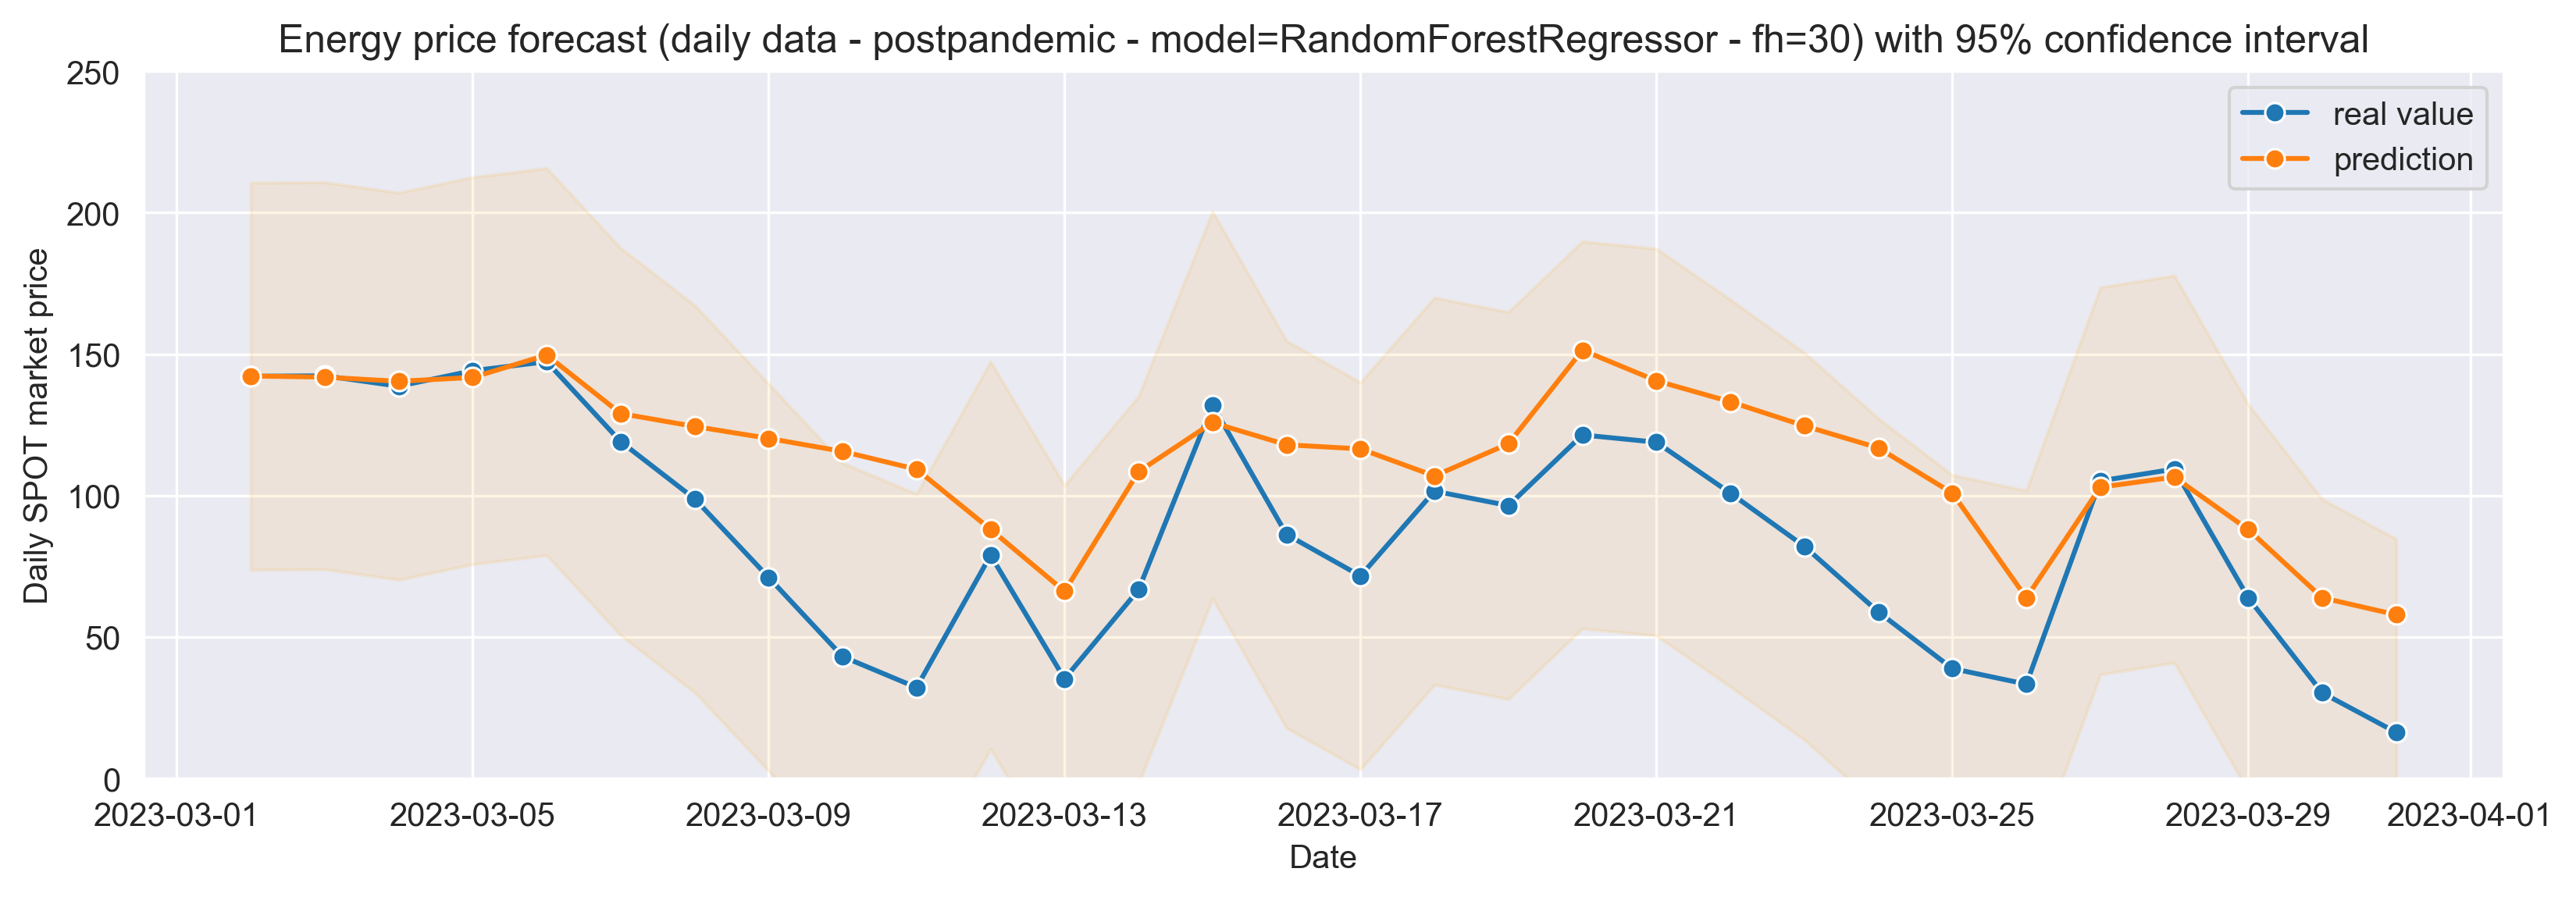
\includegraphics[scale=0.4]{images/analysis/forecast-daily-post}}
\end{figure}

Finally, let's compute the SHAP values.
%Looking at SHAP values we see similar tendencies to what seen in the pre-pandemic situation. Clean energies tend to reduce price while commodity-based generation technologies increase it. Nevertheless, the impact on the model output in the post-war situation is generally higher because the SHAP values show also larger values.
%
\begin{figure}[H]
\centering
    \begin{subfigure}{.45\textwidth}
        \centering
        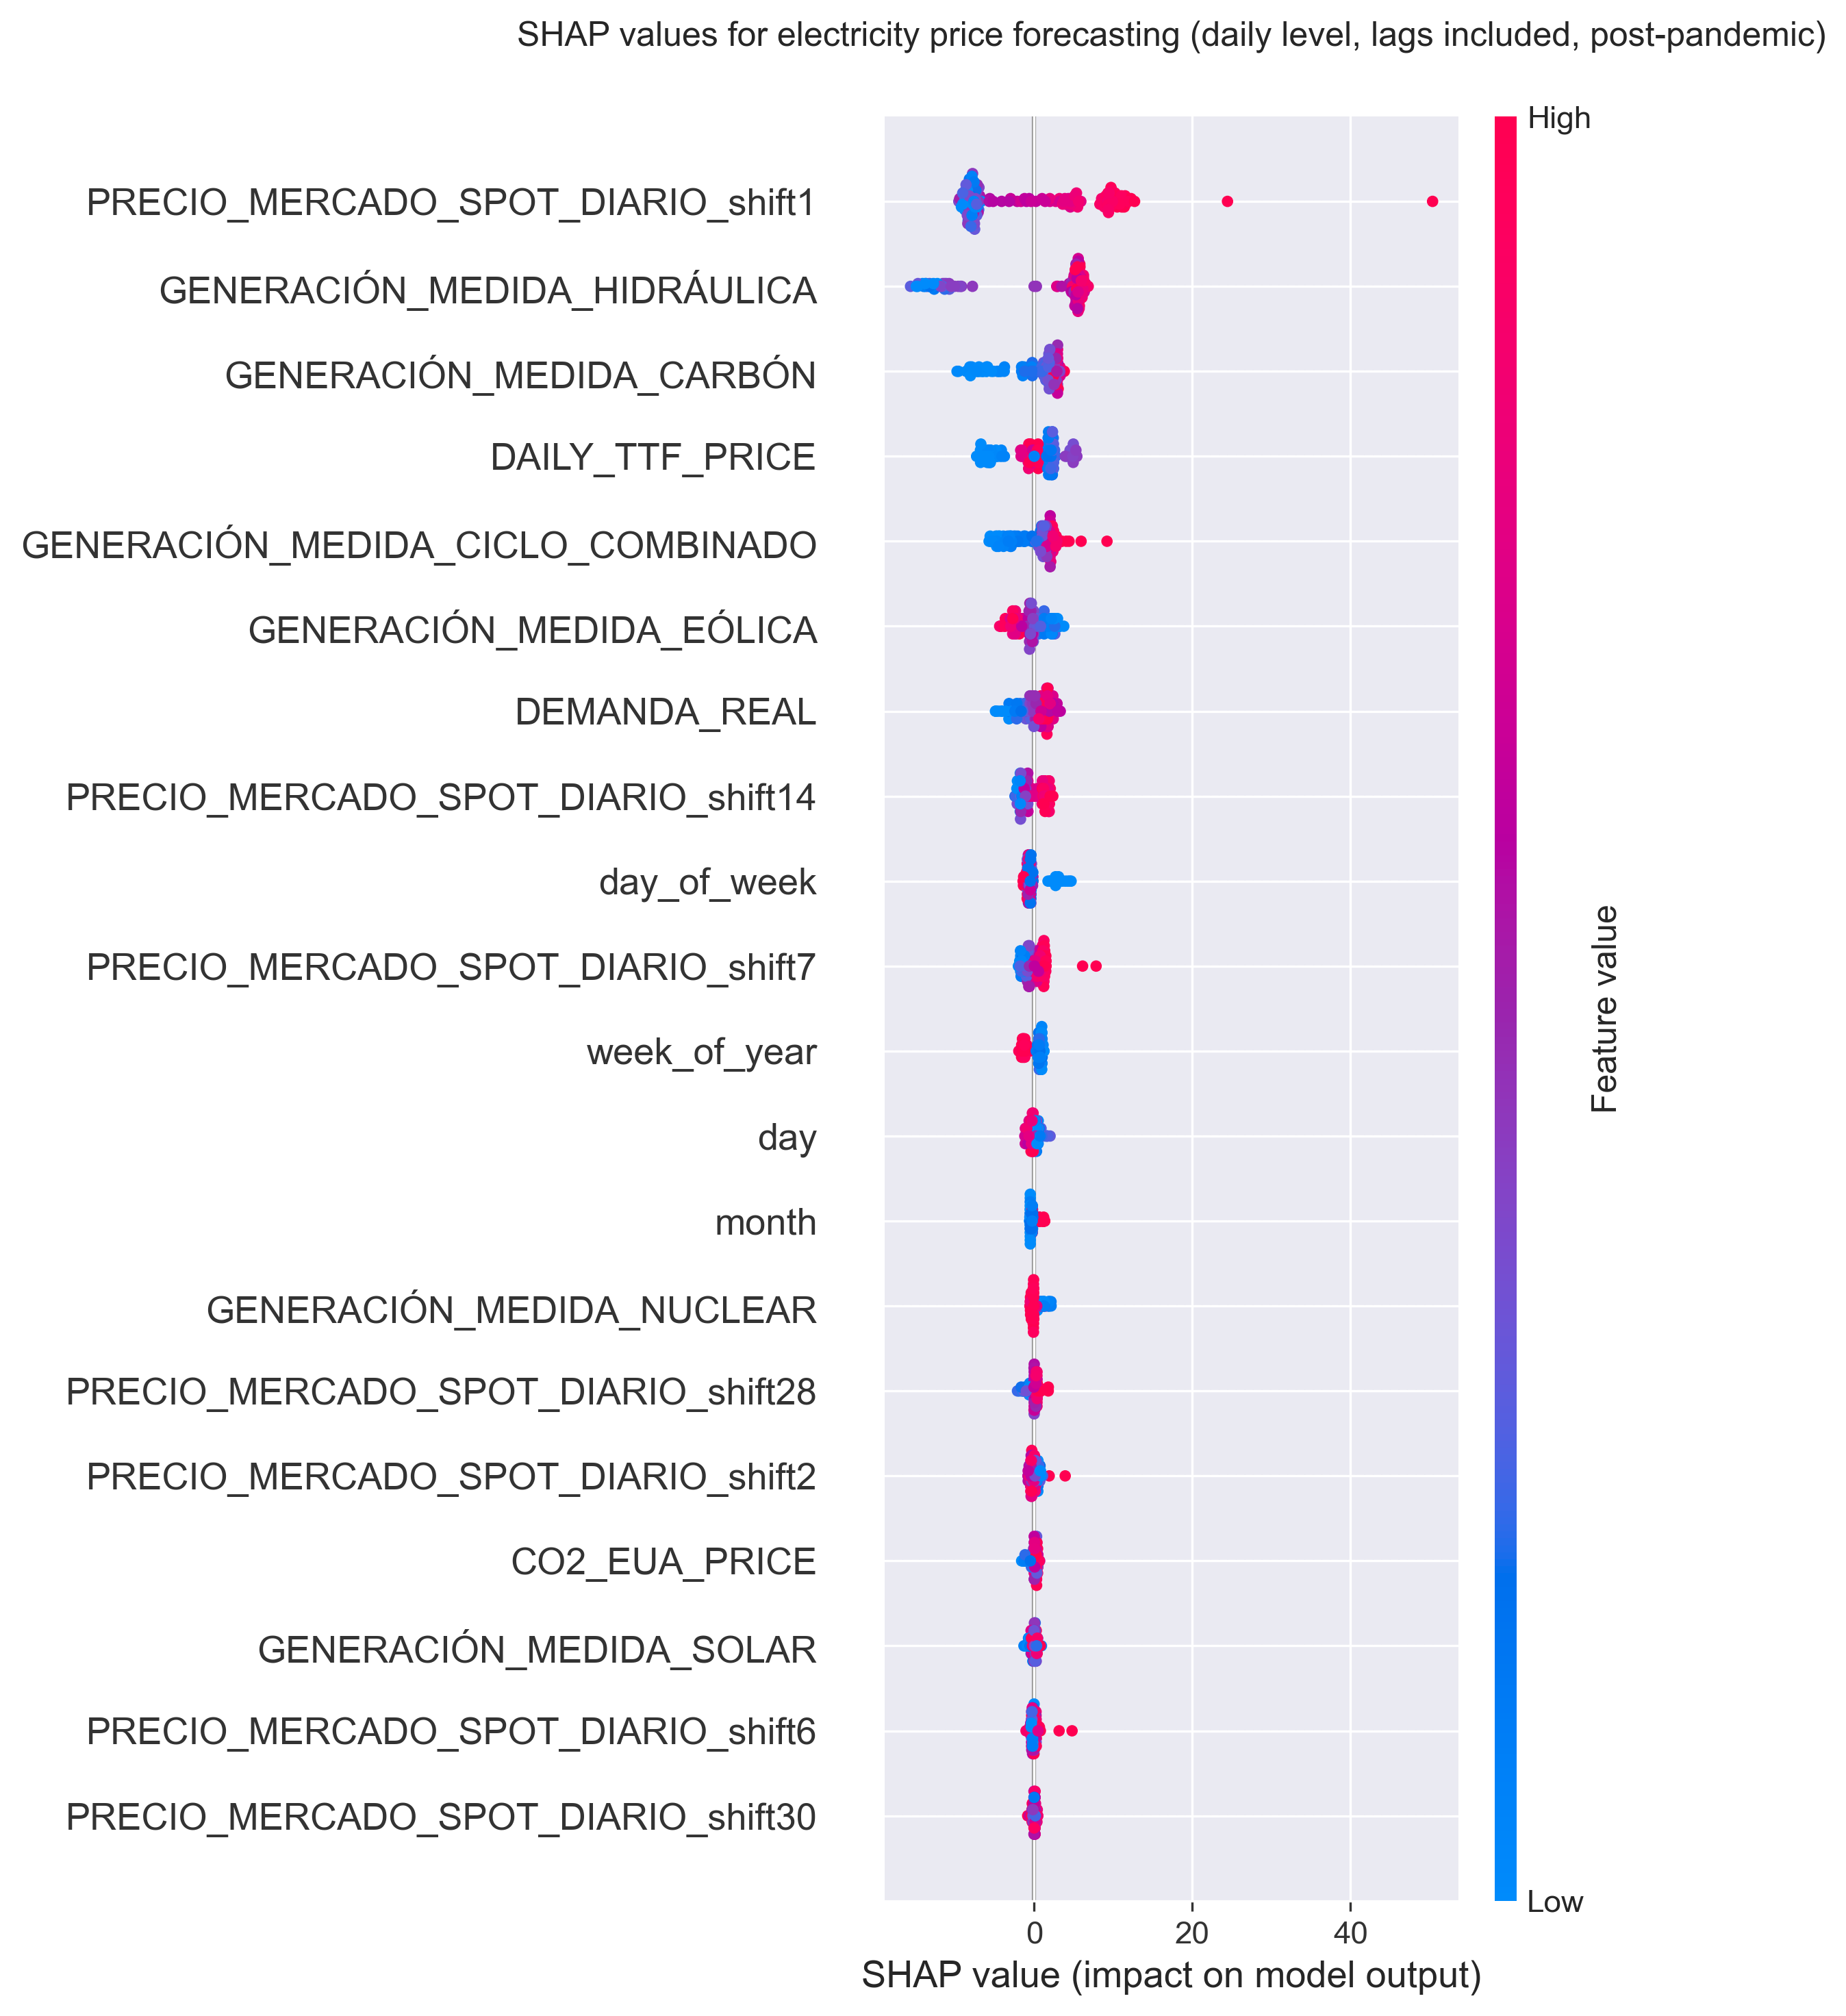
\includegraphics[width=1\linewidth]{images/analysis/shap-daily-post}
        \caption{fh=1}
    \end{subfigure}
    \begin{subfigure}{.45\textwidth}
        \centering
        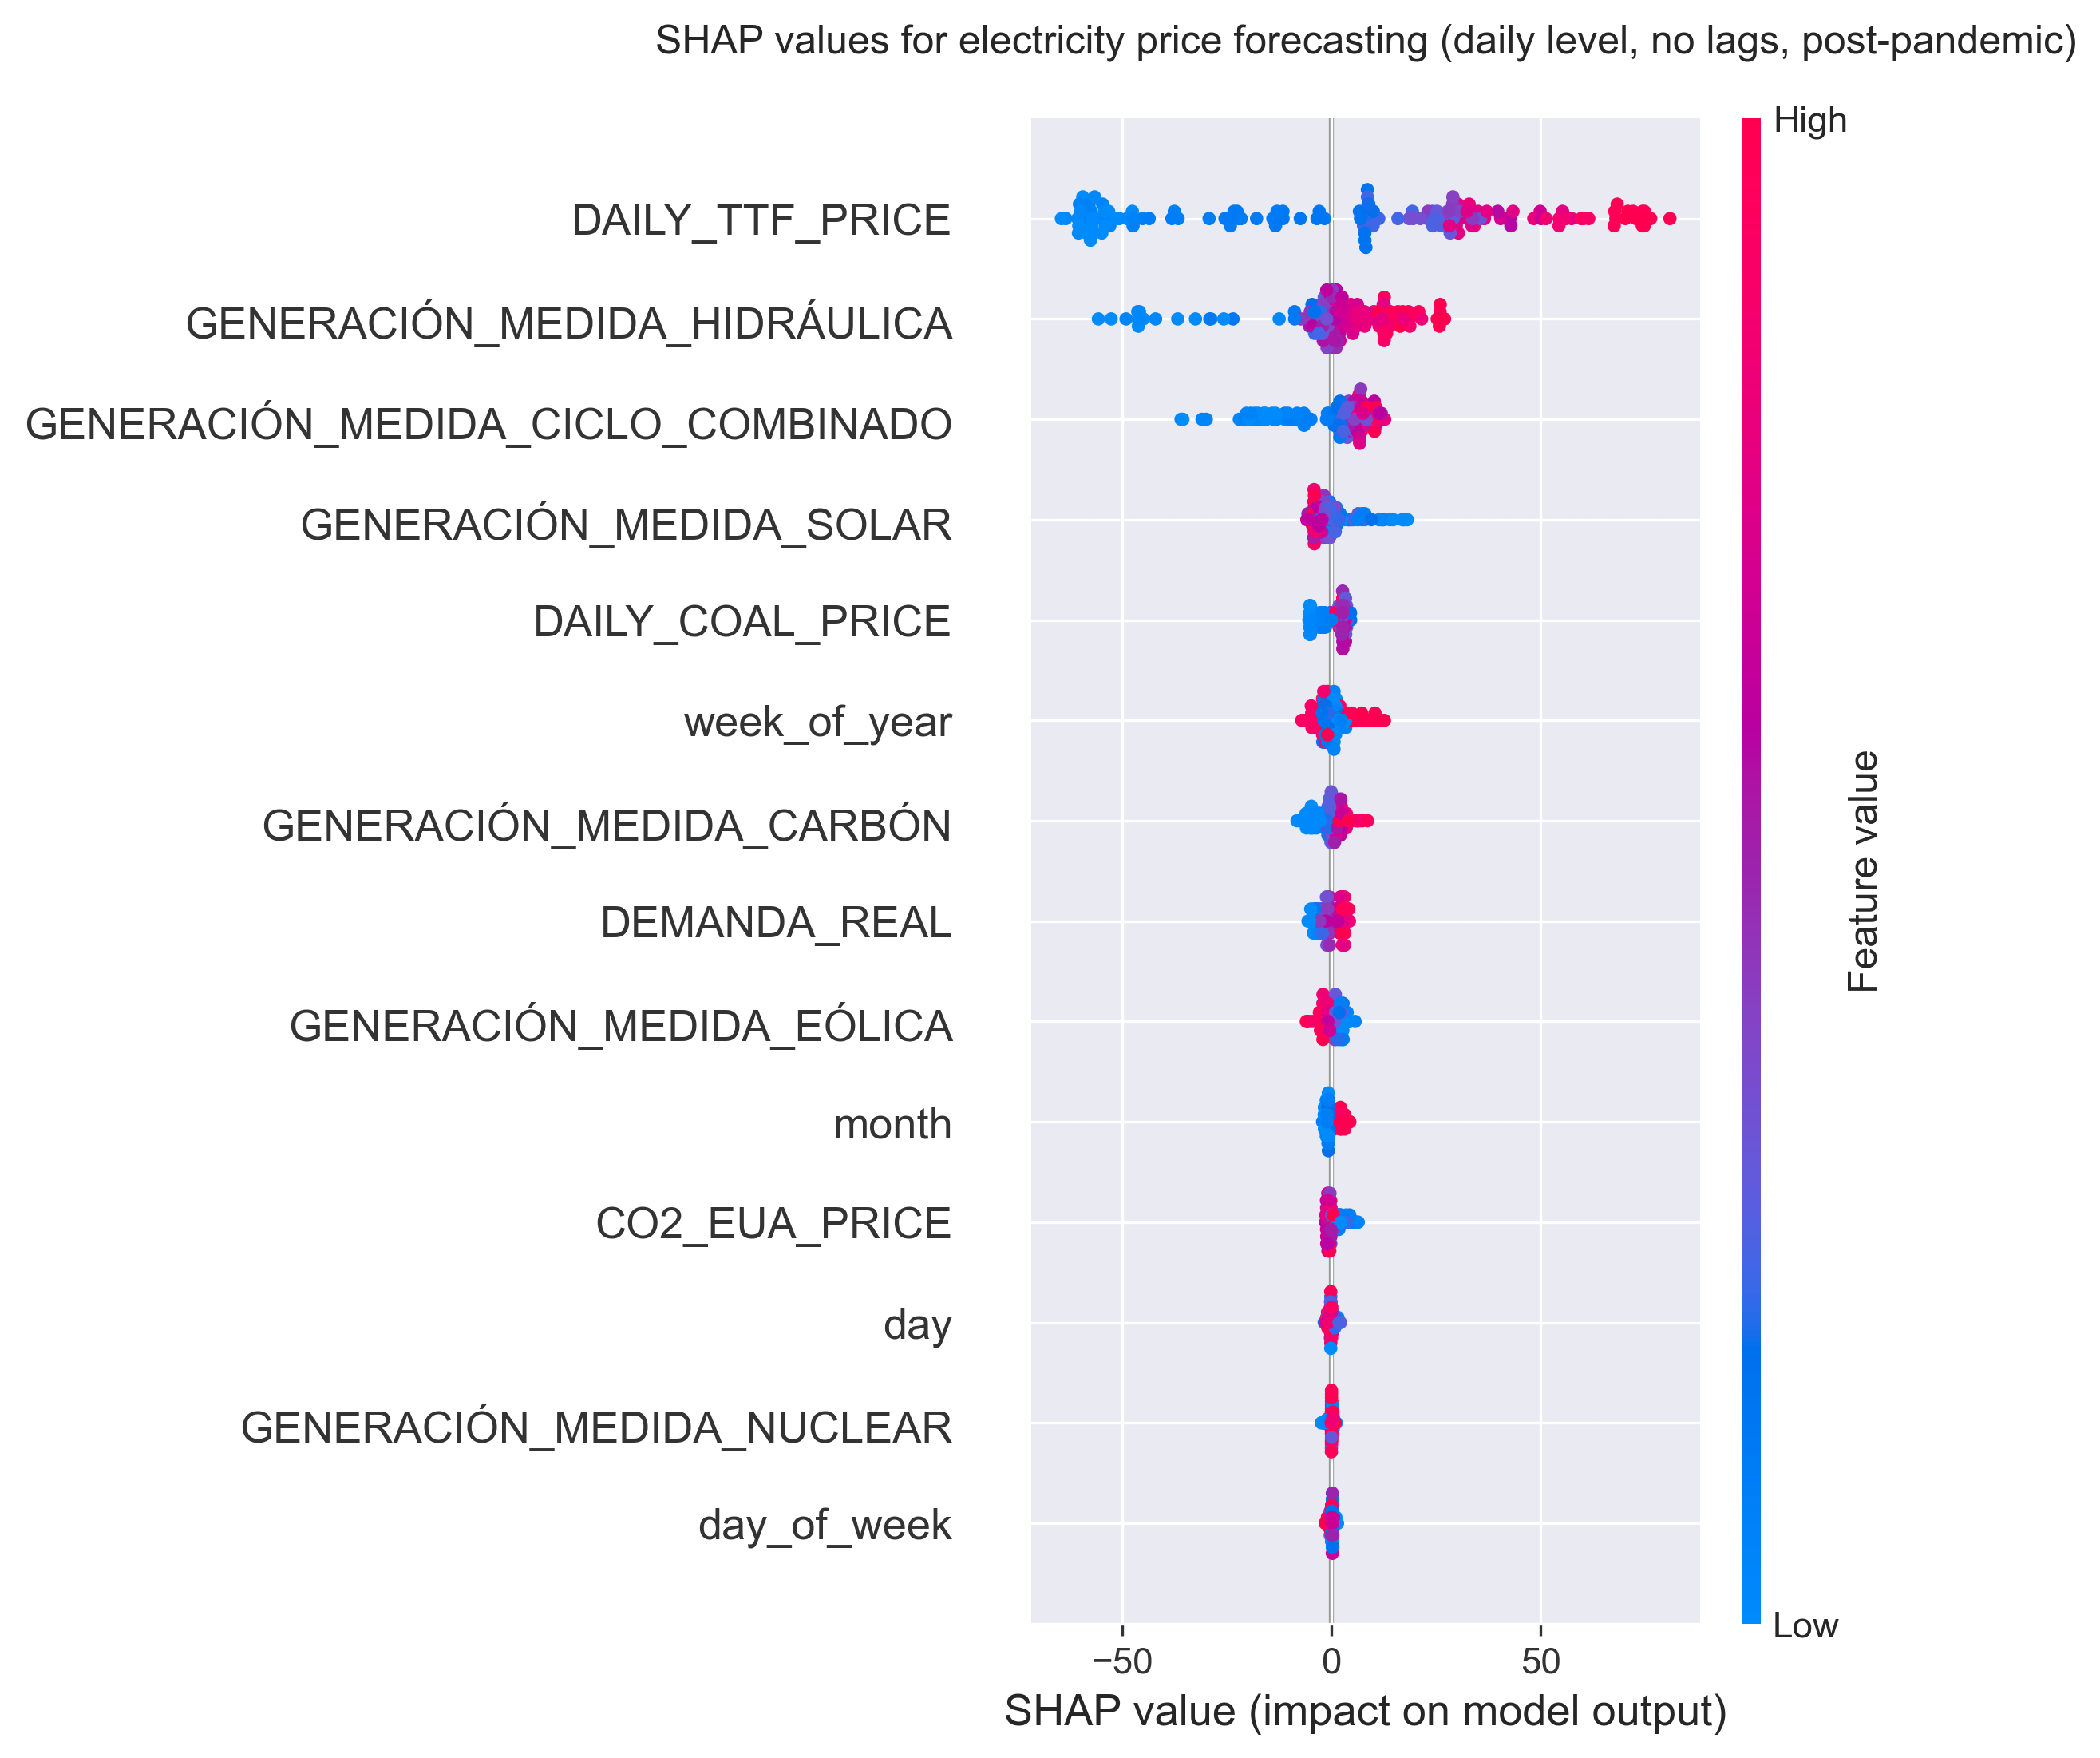
\includegraphics[width=1\linewidth]{images/analysis/shap-daily-post-nolags}
        \caption{fh=30}
    \end{subfigure}

    \caption{SHAP values for the daily post-war energy price forecasting.}
    \label{fig:shap-daily-post}
\end{figure}

Again, lag 1 is the most influencing lag. Before, the renewable technology most influencing the price was wind power, but now it changes to hydropower. Coal and combined cycle are

\subsection{Result discussion}



\section{Monthly analysis}
In the monthly level the author won't compare pre-pandemic with post-war markets as there are no enough datapoints. He will perform the study over the complete series, with data from 2014-01 to 2023-03.

The same predictors as before are used, except those related with date, which change:
\begin{itemize}
    \item \textbf{Date predictors:} Month and year.
\end{itemize}

%The best model now is the one based on Support Vector Machine

\begin{table}[H]
\centering
\begin{tabular}{@{}l|l|l@{}}
\toprule
Model & MASE  & Modelling time (s)  \\ \midrule
GBT   & 1.690  & 84.55    \\
RF    & 1.749  & 117.03   \\
kNN   & 2.662  & 108.33   \\ \bottomrule
\end{tabular}
\caption{}
\label{tab:cv-daily}
\end{table}

\begin{figure}[H]
\centering
    \caption{Final forecasting of monthly energy price.}
    \label{fig:forecast-monthly}
    \fbox{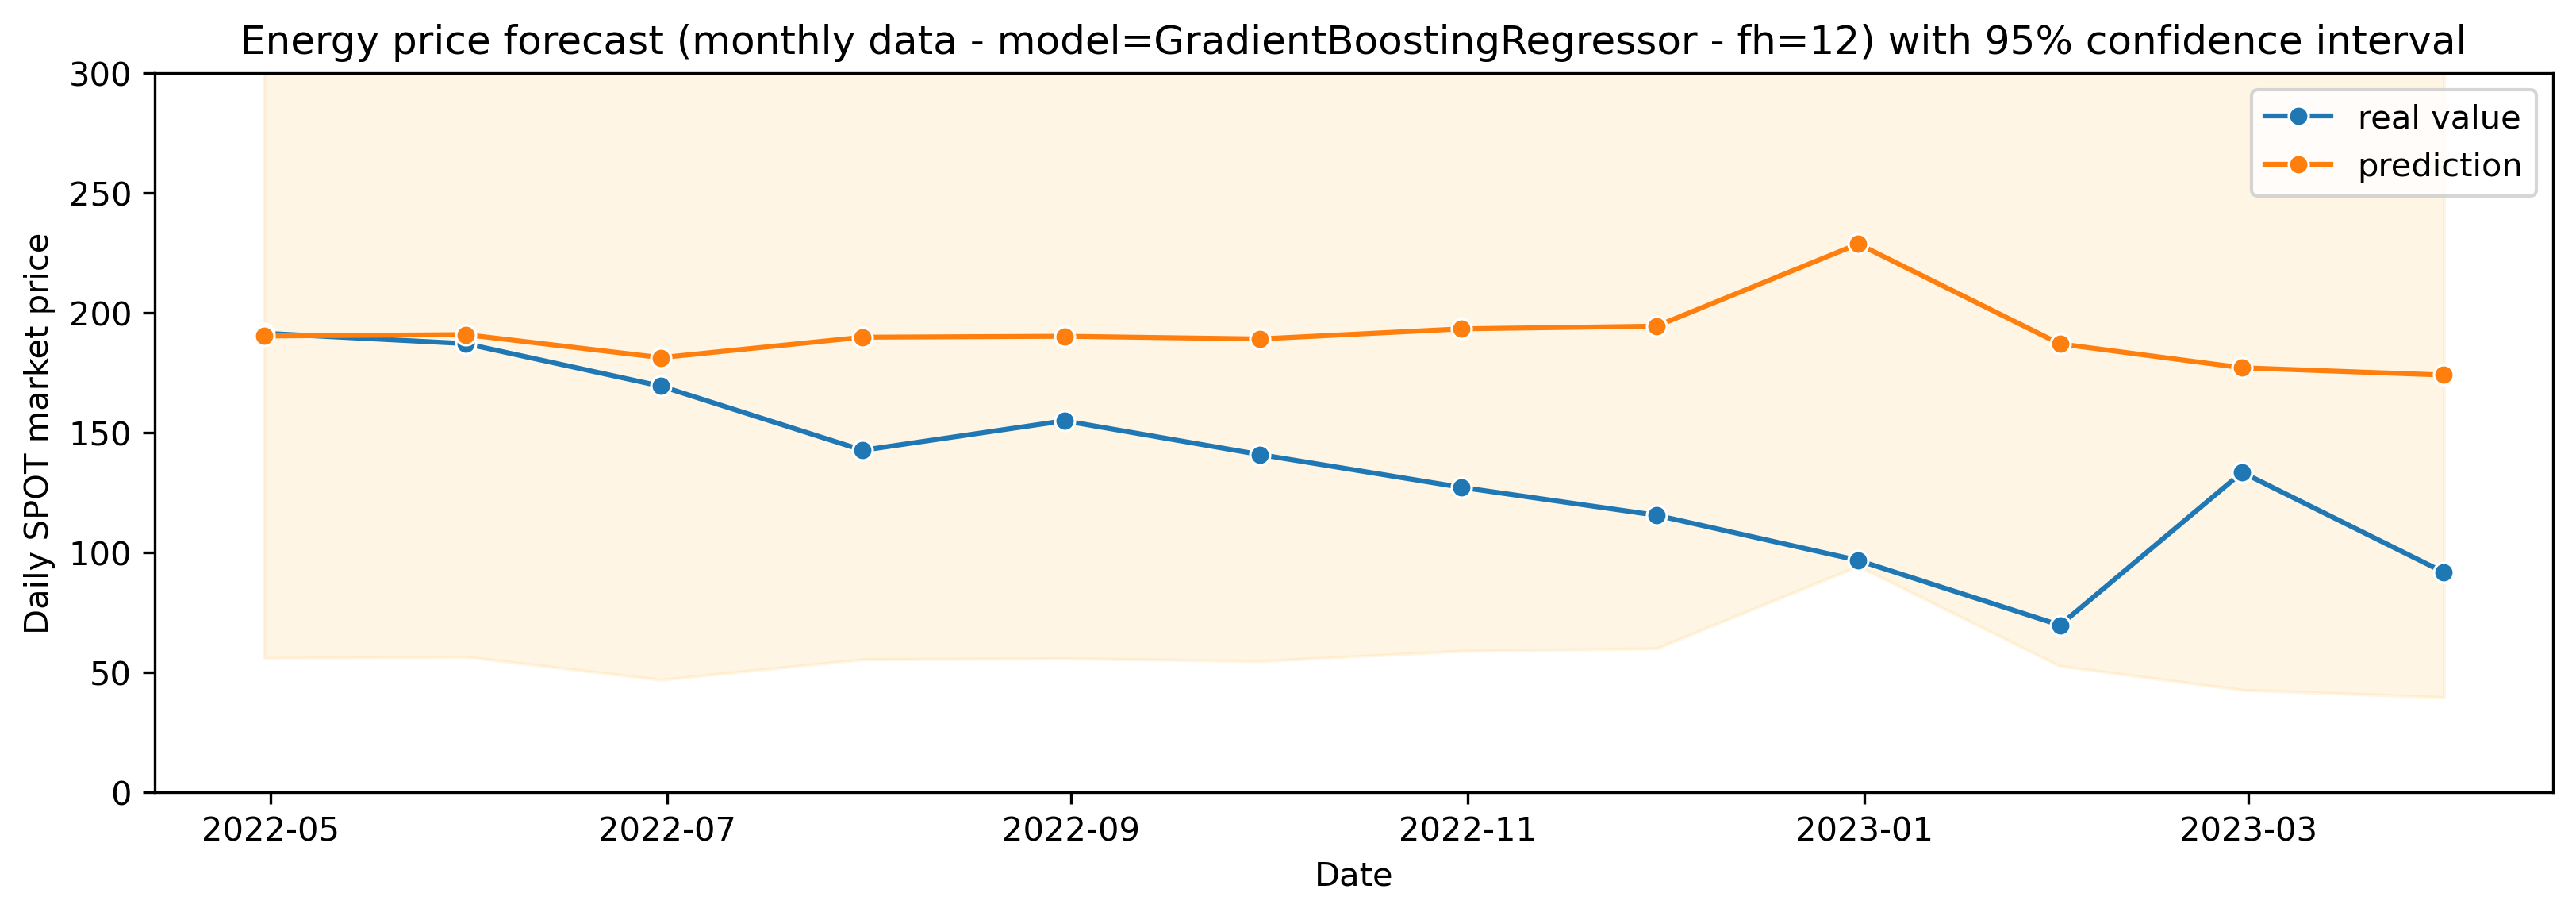
\includegraphics[scale=0.4]{images/analysis/forecast-monthly}}
\end{figure}

\begin{figure}[H]
\centering
    \begin{subfigure}{.45\textwidth}
        \centering
        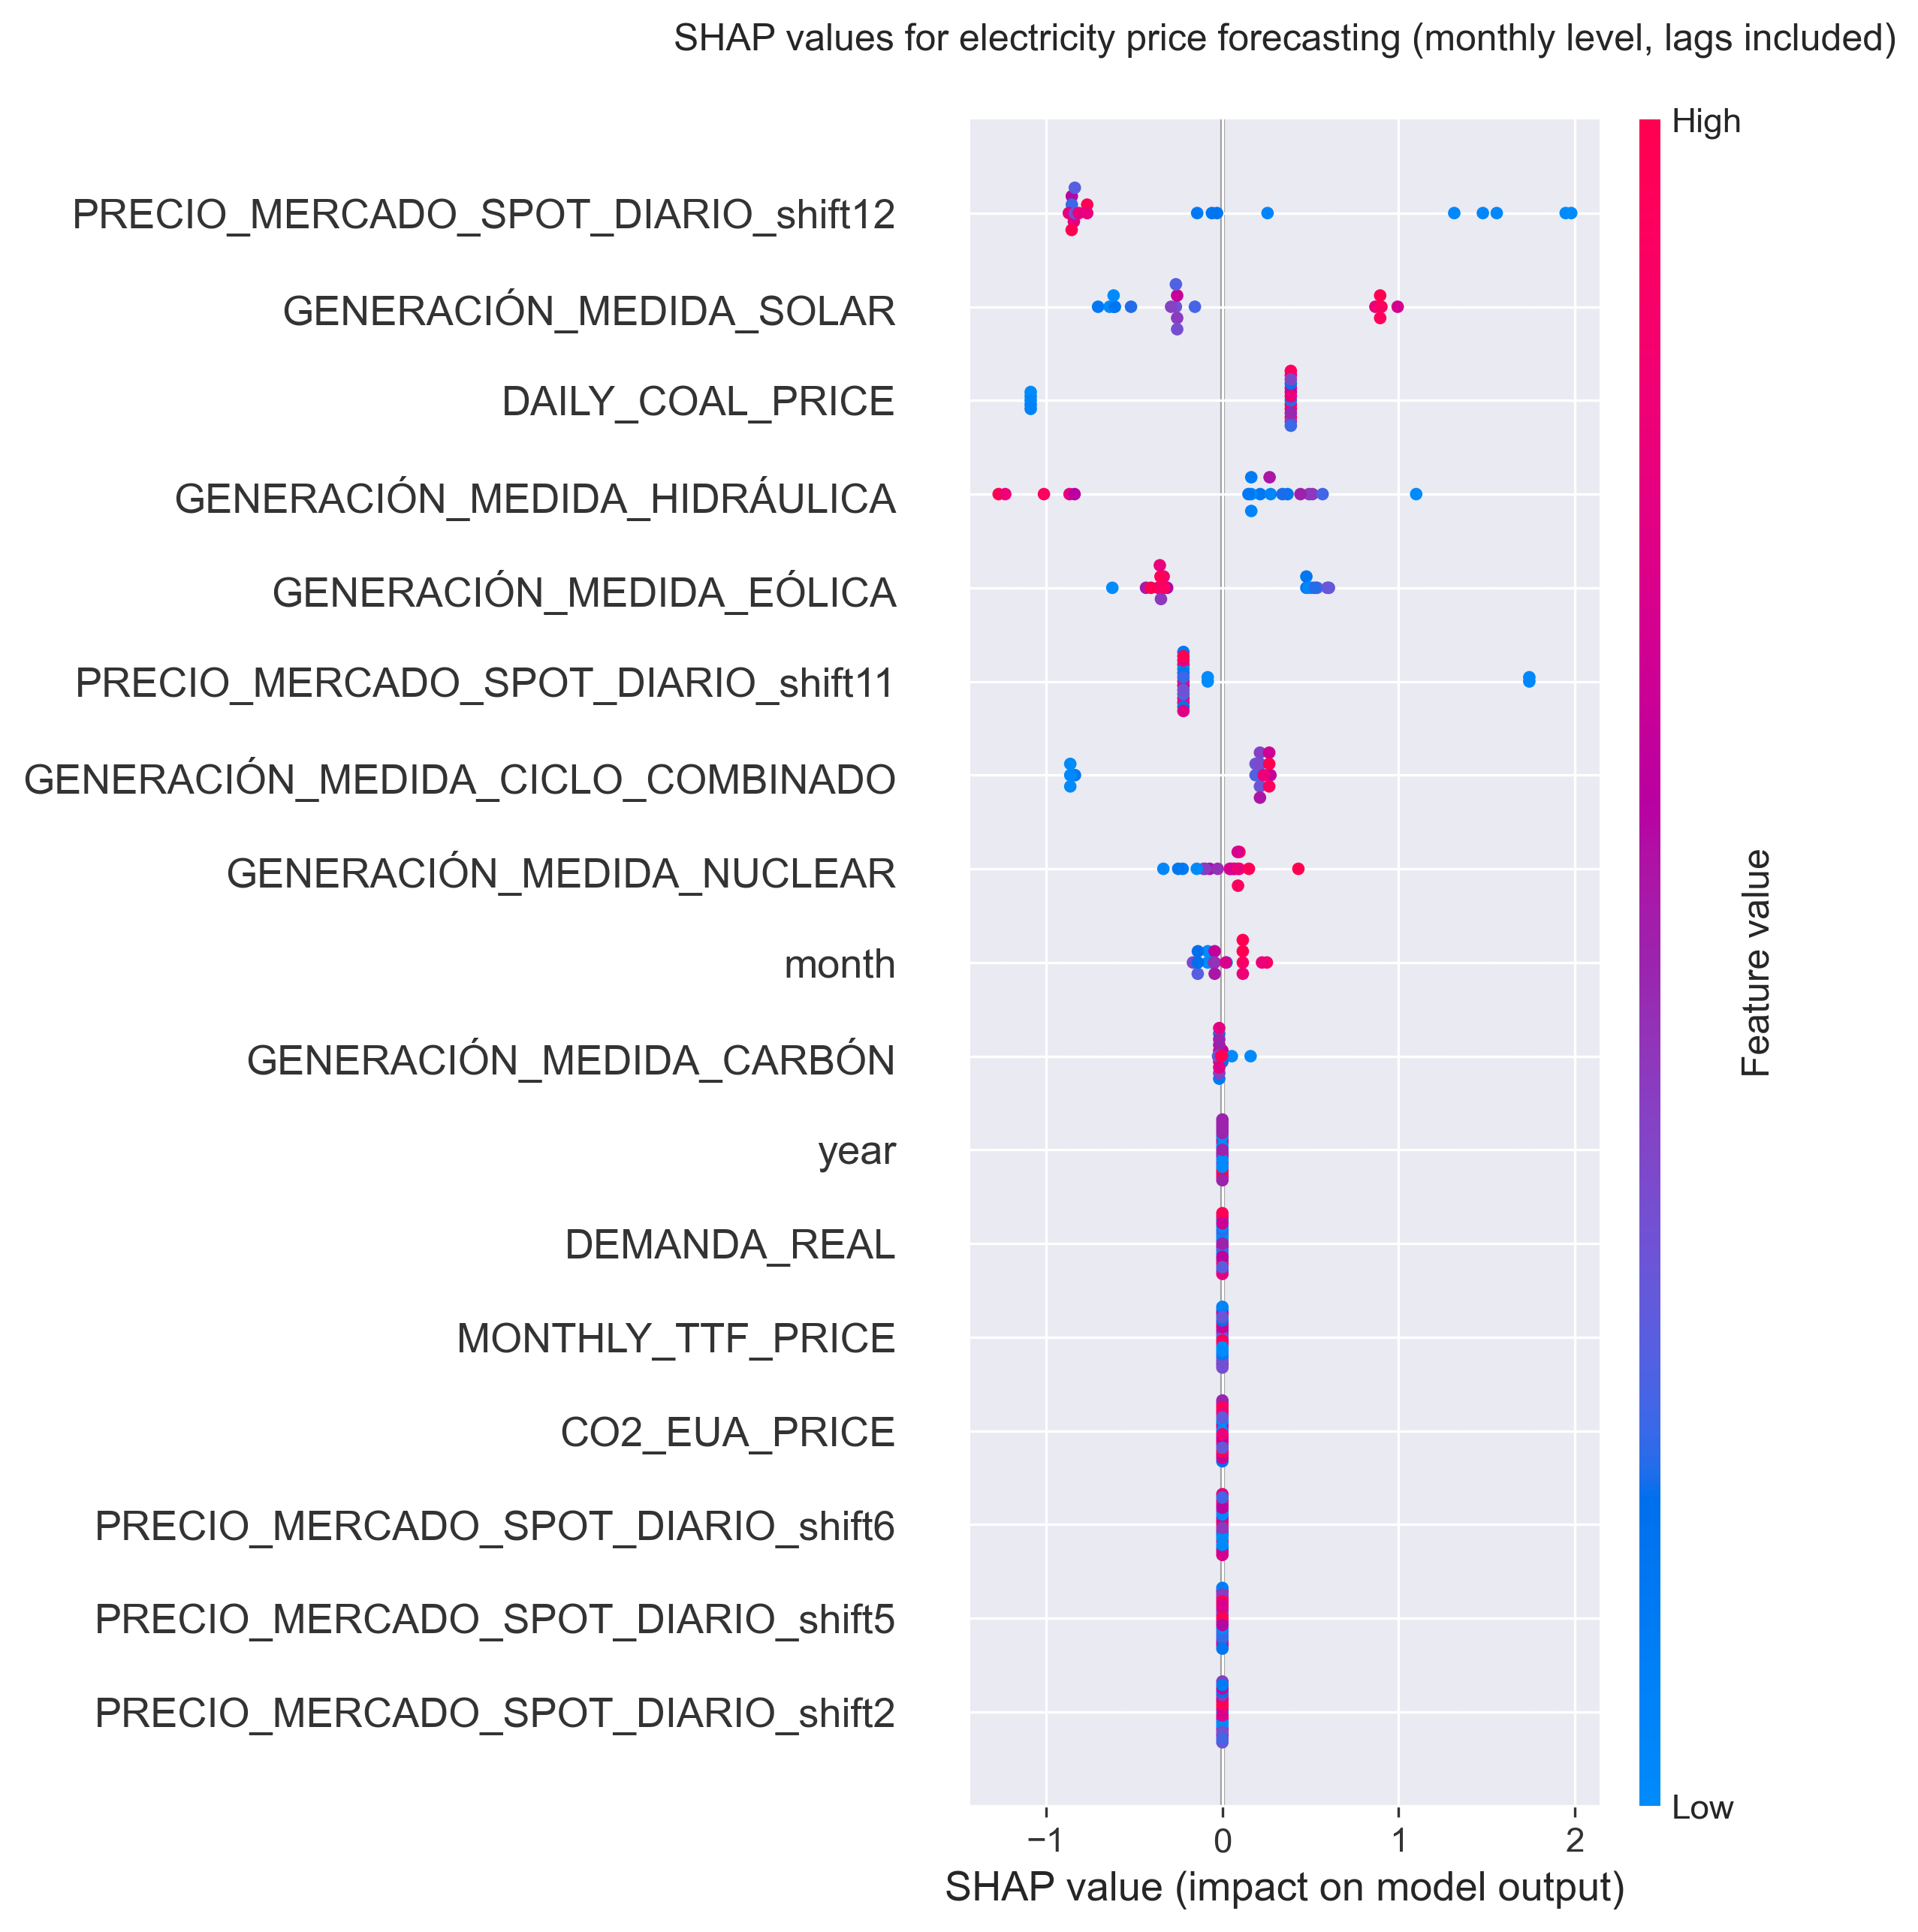
\includegraphics[width=1\linewidth]{images/analysis/shap-monthly}
        \caption{fh=1}
    \end{subfigure}
    \begin{subfigure}{.45\textwidth}
        \centering
        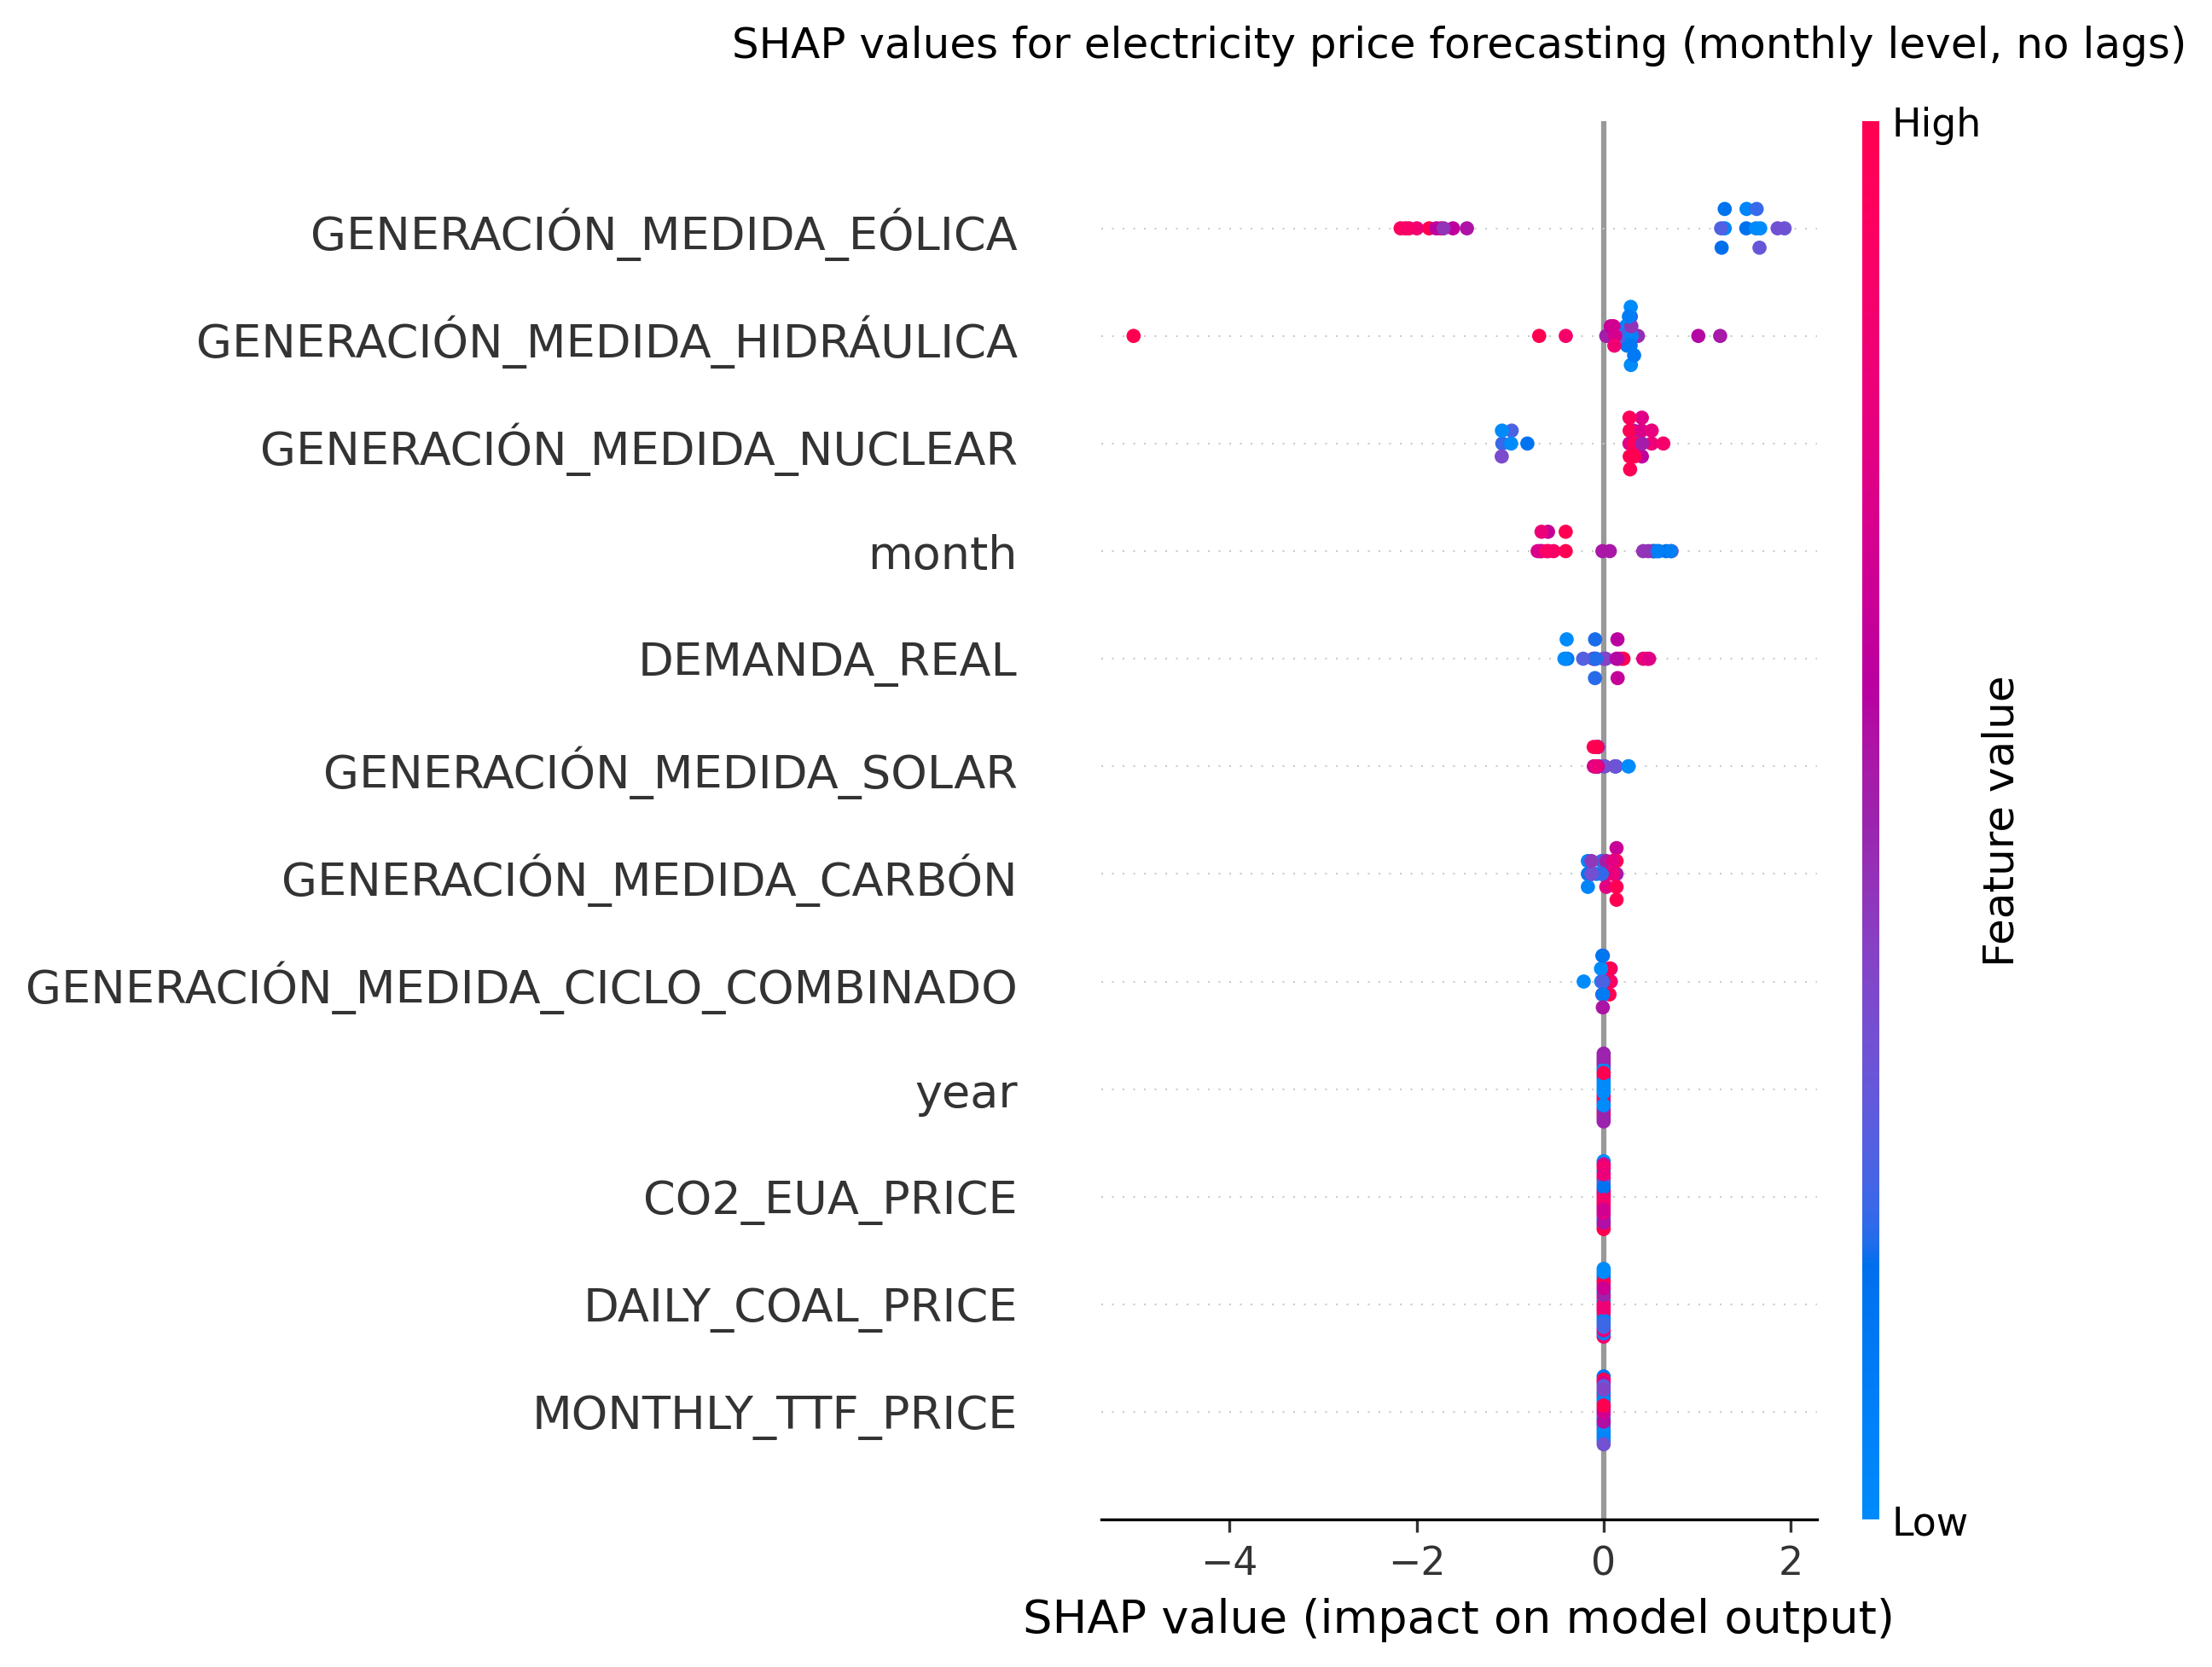
\includegraphics[width=1\linewidth]{images/analysis/shap-monthly-nolags}
        \caption{fh=12}
    \end{subfigure}

    \caption{SHAP values for the monthly energy price forecasting.}
    \label{fig:shap-monthly}
\end{figure}



\section{Yearly analysis}